\chapter{Analisi della rete}
\section{Analisi del dataset}
Il dataset considerato mostra una evidente distinzione in tre layer:
\begin{itemize}
	\item Attacchi;
	\item Messaggi;
	\item Trade.
\end{itemize}
Ognuno di questi layer è stato analizzato per un periodo complessivo di 30 giorni, producendo di fatto un differente grafo per ogni giorno e per ogni layer (90 grafi totali).\\
Il dataset è reso disponibile in due differenti formati, \texttt{csv} e \texttt{graphml}; essendo stati riscontrati dei problemi di inconsistenza tra i due formati, e a seguito di indicazioni da parte del fornitore del dataset, abbiamo deciso di considerare unicamente il formato \texttt{graphml}.\\
La rete analizzata risulta essere un multi-grafo diretto multi-layer. Considerato il fatto che la maggior parte delle misure di centralità di una rete sono pensate per grafi (e non per multi-grafi), è stato deciso di trasformare la rete in un grafo diretto pesato, dove il peso di un arco tra due nodi rappresentasse il numero di archi che connette i due nodi nel multi-grafo. Questa operazione è stata eseguita per ognuno dei 90 grafi, in modo da mantenere inalterati layer e \textit{timeslice}. Questa scelta ha permesso di ridurre drasticamente i tempi computazionali per le varie analisi che verranno presentate, preservando l'informazione grazie al peso degli archi.\\
È stata inoltre prodotta per ogni layer una versione aggregata sui 30 giorni, in modo da fornire una visone complessiva della rete e delle relazioni tra i vari nodi.
Tutti e tre i layer presentano archi orientati e con un \textit{timestamp}: esso è stato rimosso durante il passaggio a grafo pesato, ma è stato utilizzato per alcune analisi presentate in seguito.\\
Sono stati anche rilevati dei \textit{sefl-loop} nel layer dei messaggi: dato che in Travian non offre la possibilità di inviare un messaggio a se stessi, abbiamo deciso di rimuovere questi archi, anche considerando il fatto che la loro numerosità non era statisticamente rilevante ($0.03\%$).

Dall'analisi delle reti aggregate sui 30 giorni, riportata nella Tabella \ref{tab:summary}, notiamo come vi sia una predominanza di attività di attacco tra giocatori, seguita dai messaggi e dagli scambi. Il trand si conferma anche per quanto riguarda il numero di nodi attivi: troviamo un totale di nodi coinvolti in attività di combattimento superiore al numero di quelli che si scambiano messaggi o commerciano. Notiamo inoltre che unendo le tre reti in un unico grafo, otteniamo un numero di nodi superiore rispetto alle 3 reti separate. Ciò indica la presenza di giocatori che sono completamente estranei ad una di queste tre attività (\textit{e.g.}, soggetti che attaccano senza mai commerciare).\\
Il diametro della rete, valore rilevante esclusivamente per il layer dei messaggi, indica che il numero massimo di giocatori da cui deve passare l'informazione affinché venga trasmessa tra due qualunque nodi è molto contenuto, pari solo a 9.\\
Il numero medio di vicini ci mostra come, per quanto riguarda gli attacchi, vi sia la tendenza a selezionare bersagli preferenziali, concentrando gli attacchi verso quei villaggi che hanno già verificato essere proficui. Al contrario, l'elevato valore per quanto riguarda gli scambi evidenzia come il mercato sia “globalizzato”, si tende a scambiare la propria merce con chiunque sia in grado di offrire in cambio un compenso ritenuto adeguato, senza la creazione di  “scambi ricorrenti”.\\
Il valore della reciprocità media esprime quanto nel grafo siano presenti collegamenti bidirezionali tra nodi. È apprezzabile come questo valore risulti essere estremamente elevato per quanto riguarda gli scambi (in quanto concepiti come vendita bidirezionale) e per i messaggi. Nel grafo degli attacchi troviamo un compattamento diametralmente opposto: solo pochi giocatori rispondono agli attacchi. Questo è probabilmente dovuto al fatto che i villaggi attaccati siano solitamente più deboli degli attaccanti, e non sarebbero quindi in grado di portare a termine con successo un attacco nei confronti degli assalitori.
\begin{table}[h]
	\centering
	\caption{Analisi macroscopica dei vari layer del dataset aggregati sui 30 giorni.}
	\begin{tabular}{|c|c|c|c|c|}
		\hline 
		Misura & Attacks & Messages & Trades & All \\ 
		\hline 
		\# Nodi & 4418 & 3092 & 2648 & 4612 \\ 
		\hline 
		\# Archi & 632391 & 380794 & 269483 & 1282668 \\ 
		\hline 
		Diametro & / & 9 & / & / \\ 
		\hline 
		Numero medio di vicini & 3.98 & 43.51 & 89.89 & / \\ 
		\hline 
		Reciprocità media & 0.039 & 0.704 & 0.938 & / \\ 
		\hline 
	\end{tabular} 
	\label{tab:summary}
\end{table}

\subsection{Analisi del grado}
\label{subsec:grado}
In Figura \ref{fig:degree} sono riportate le distribuzioni di in-degree, out-degree e grado complessivo dei vari layer della rete. Dalle distribuzioni sono stati rimossi quei nodi considerati \textit{outlier}, ovvero quei nodi che si discostano oltre 3 volte dalla deviazione standard del \textit{fitting} dei dati con una distribuzione normale (per le distribuzioni di tali nodi, consultare l'Appendice A). I dati mostrano un andamento standard, con un elevato numero di nodi con grado contenuto e una percentuale minoritaria di nodi con alto grado.\\
\begin{figure}[p!]
	\begin{tabular}{ccc}
		\subfloat[Attacks in degree]{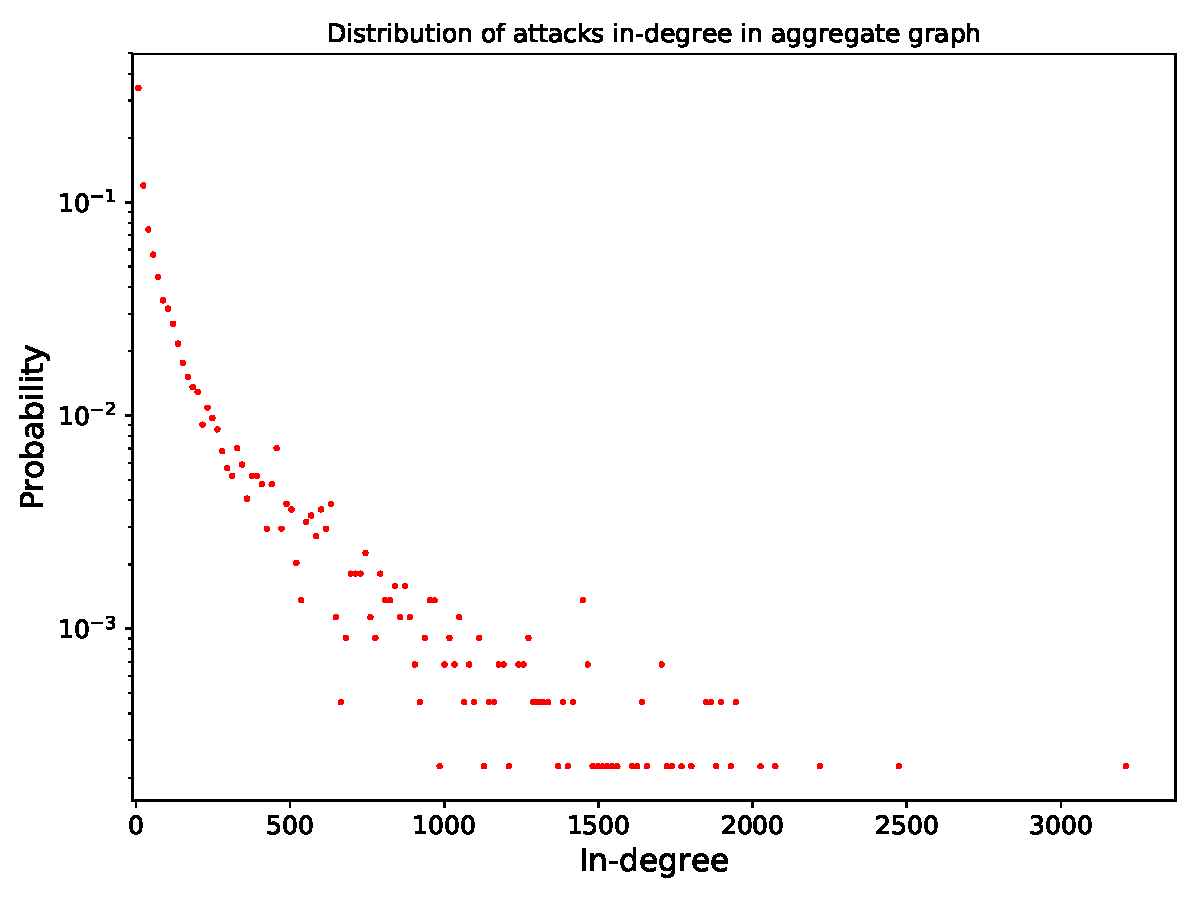
\includegraphics[width = 1.5in]{images/Aggregate/Degree/attacks_in_degree}} &
		\subfloat[Attacks out degree]{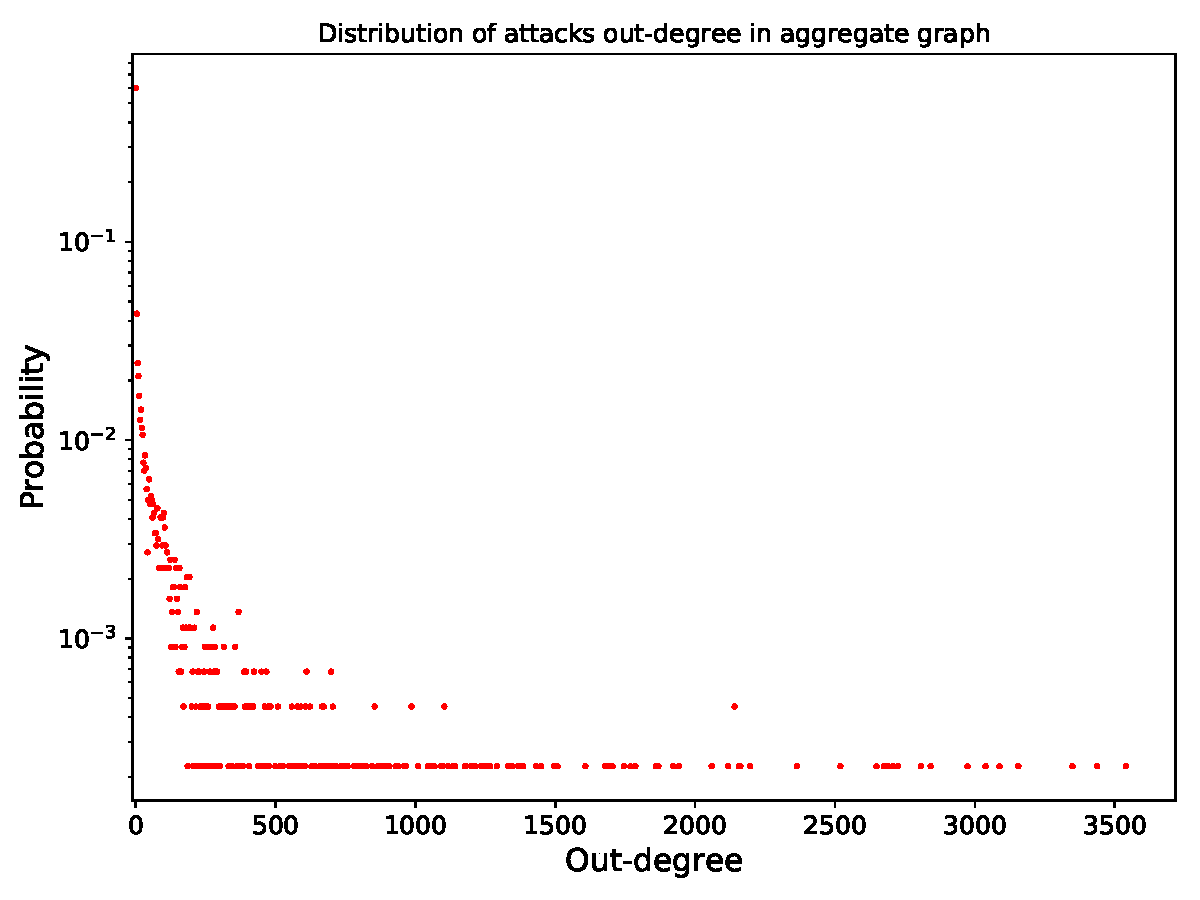
\includegraphics[width = 1.5in]{images/Aggregate/Degree/attacks_out_degree}} &
		\subfloat[Attacks total degree]{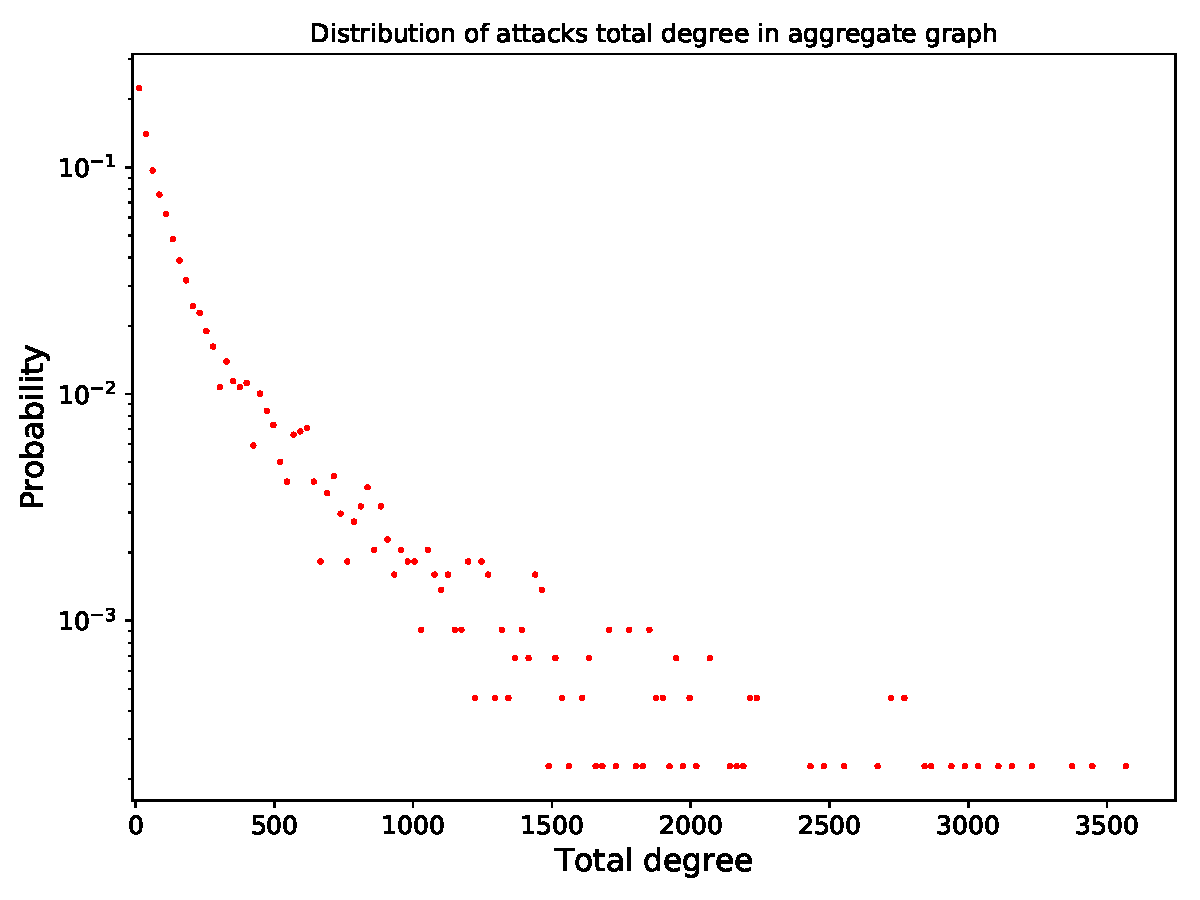
\includegraphics[width = 1.5in]{images/Aggregate/Degree/attacks_total_degree}}\\
		\subfloat[Messages in degree]{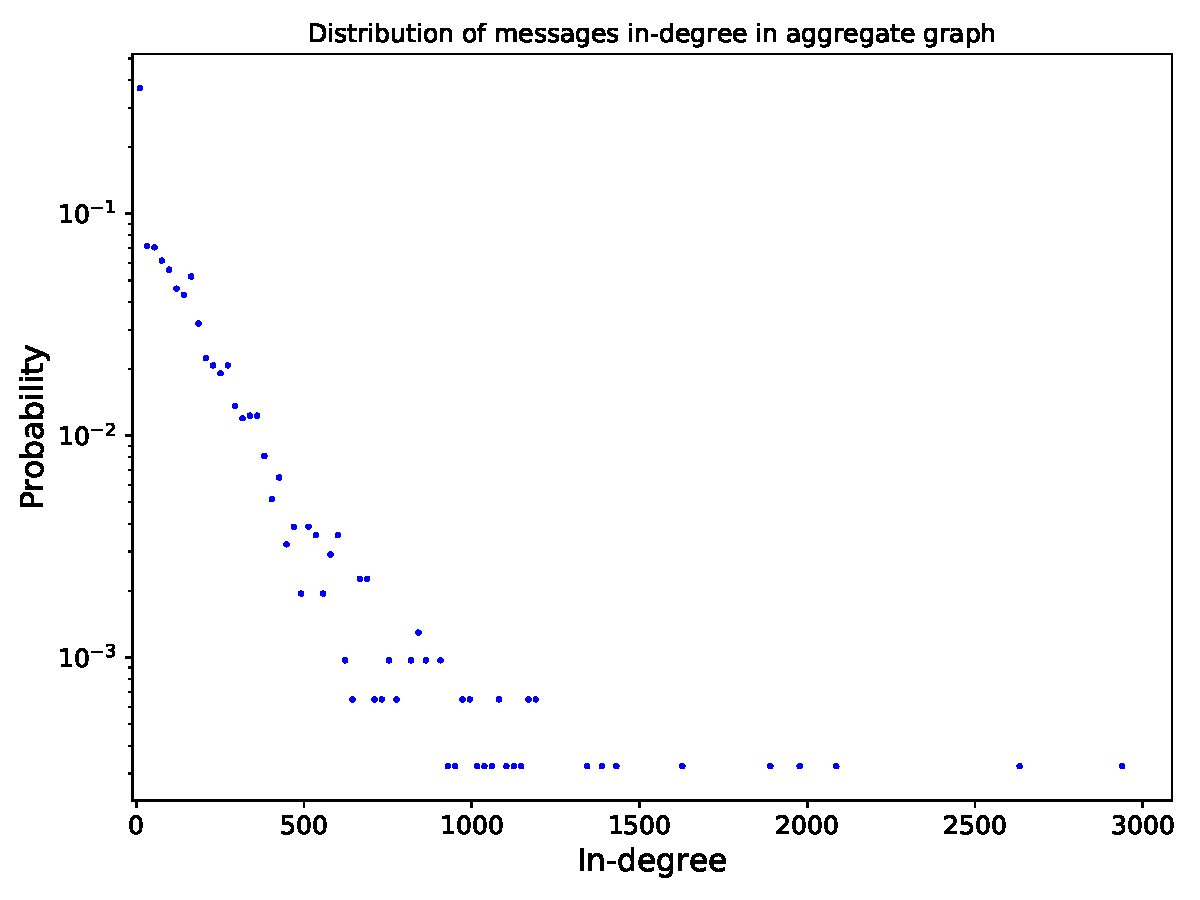
\includegraphics[width = 1.5in]{images/Aggregate/Degree/messages_in_degree}} &
		\subfloat[Messages out degree]{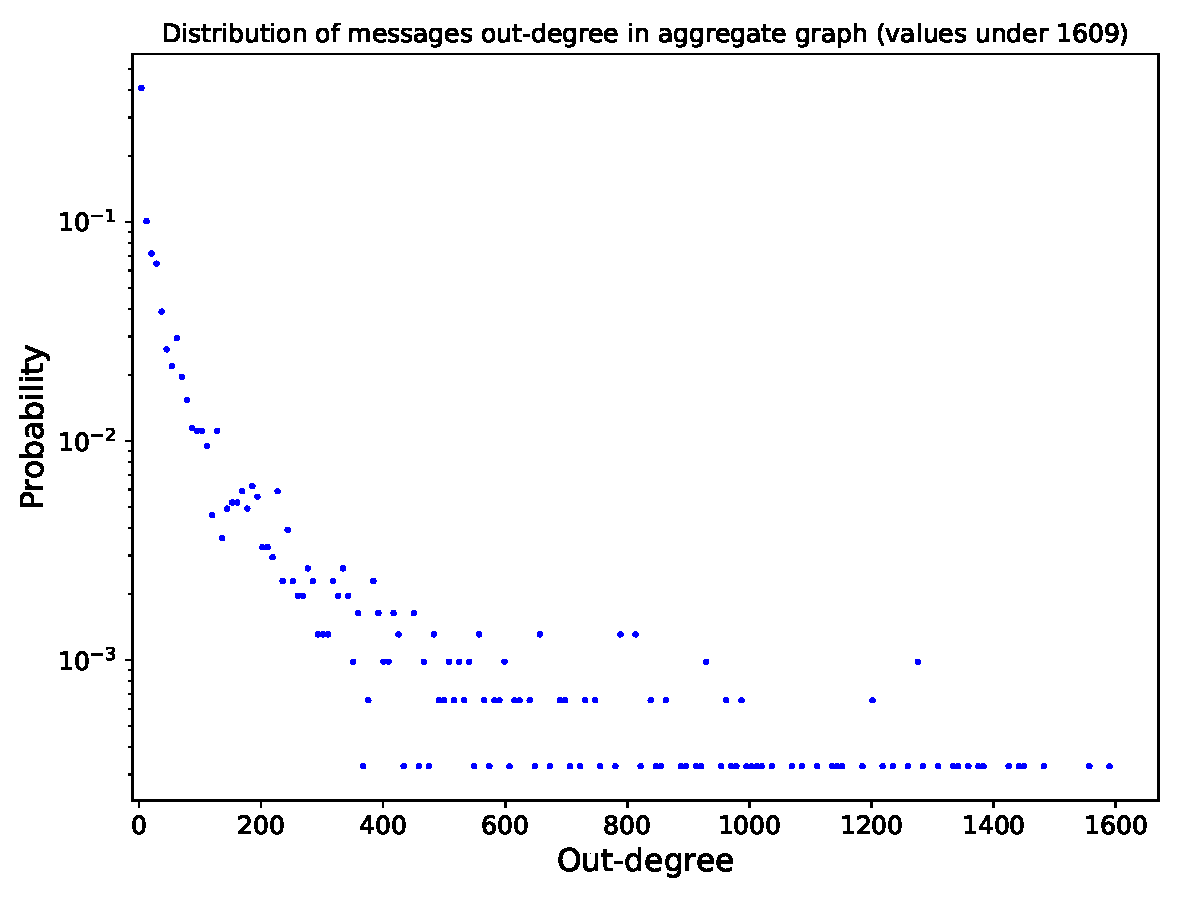
\includegraphics[width = 1.5in]{images/Aggregate/Degree/messages_out_degree}} &
		\subfloat[Messages total degree]{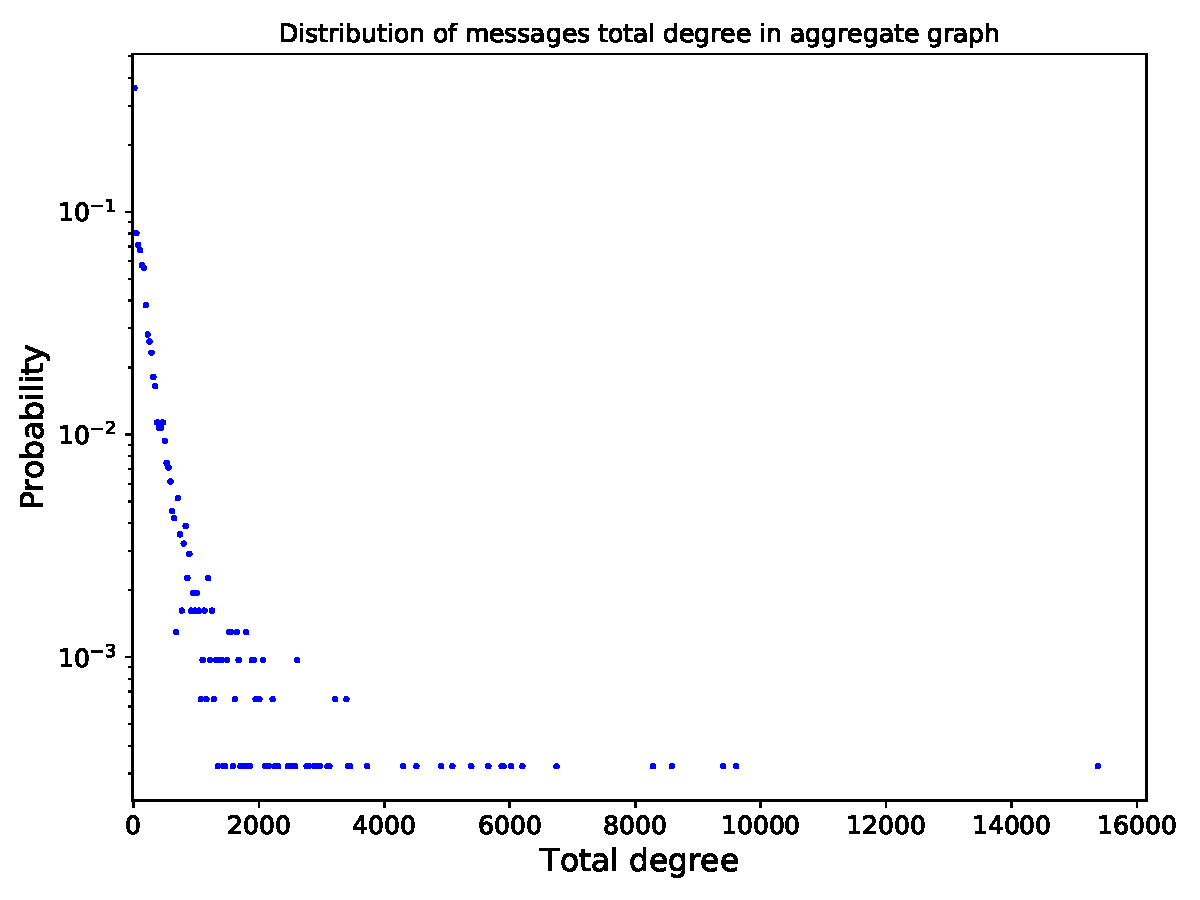
\includegraphics[width = 1.5in]{images/Aggregate/Degree/messages_total_degree}}\\
		\subfloat[Trades in degree]{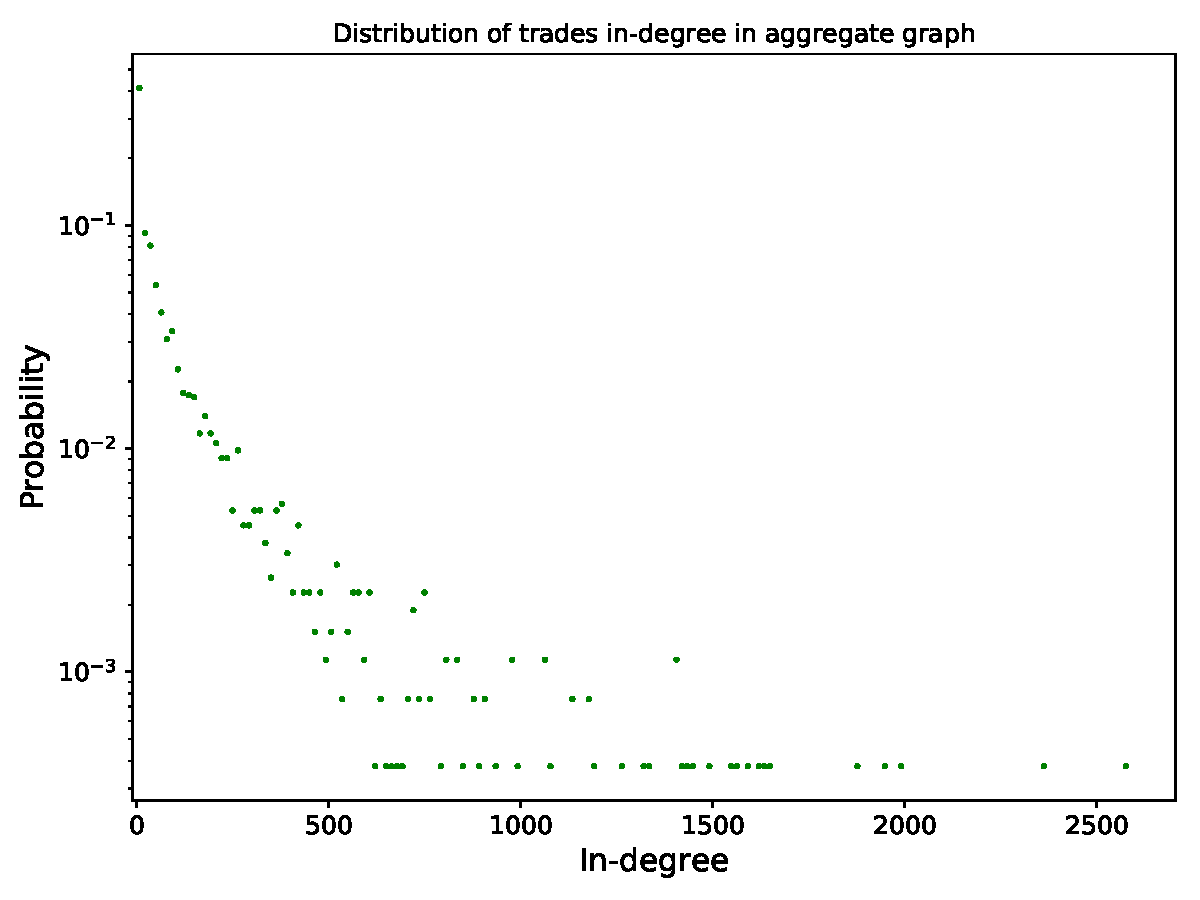
\includegraphics[width = 1.5in]{images/Aggregate/Degree/trades_in_degree}} &
		\subfloat[Trades out degree]{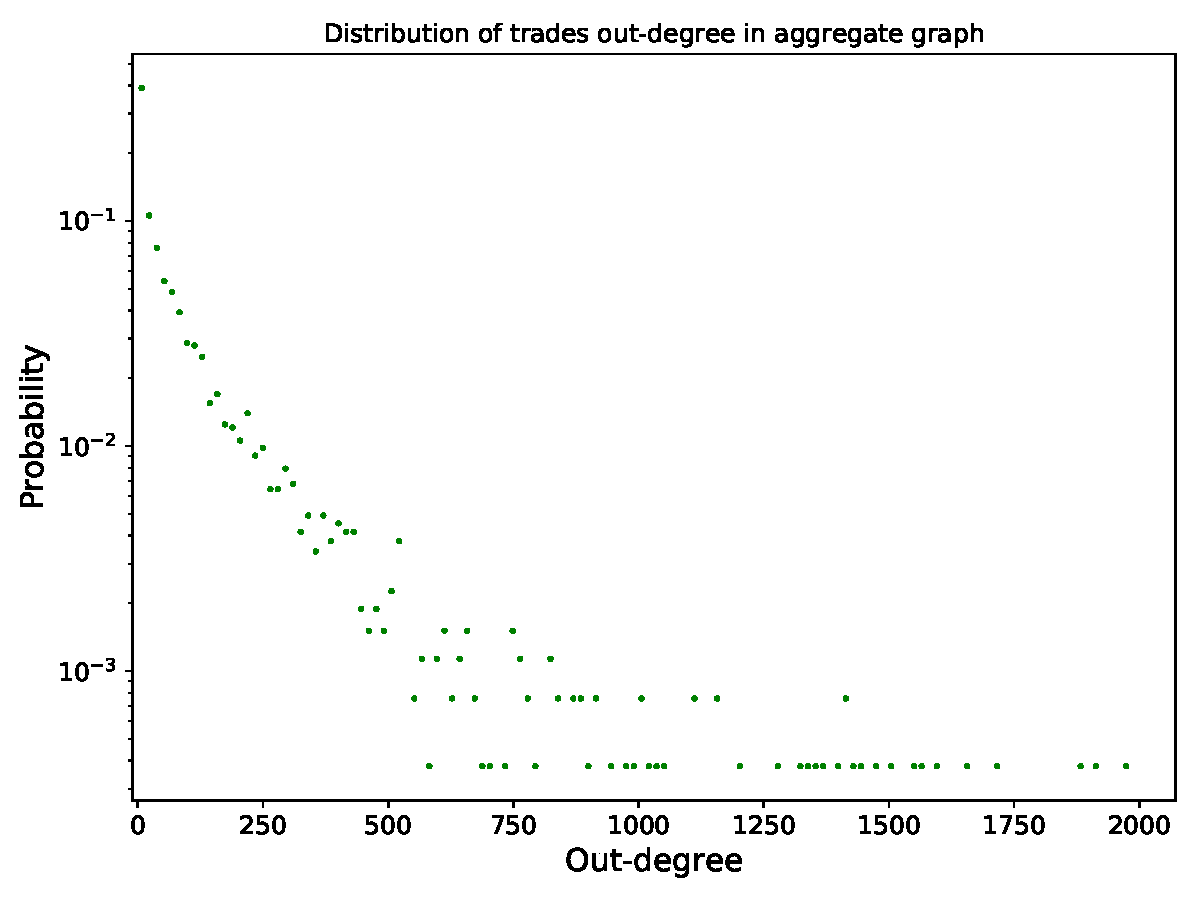
\includegraphics[width = 1.5in]{images/Aggregate/Degree/trades_out_degree}} &
		\subfloat[Trades total degree]{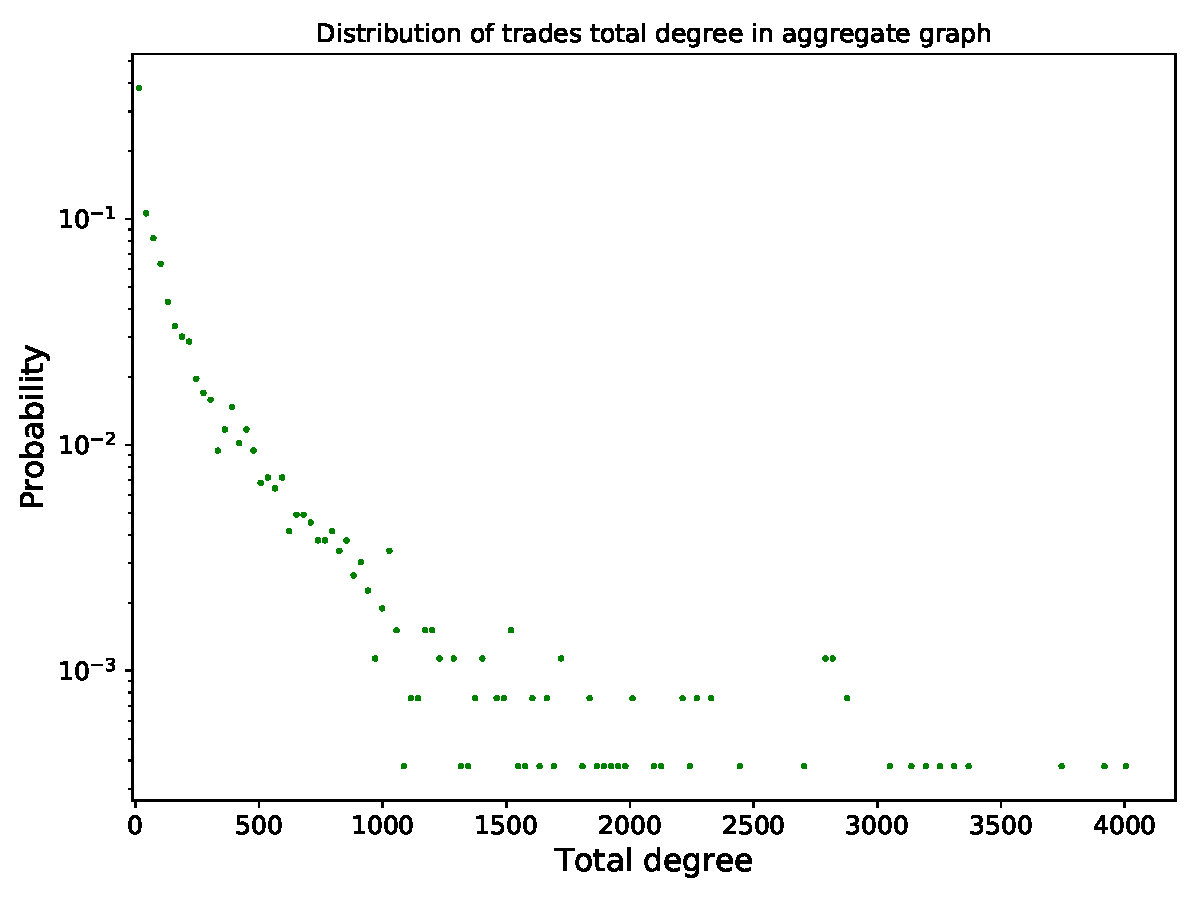
\includegraphics[width = 1.5in]{images/Aggregate/Degree/trades_total_degree}}
	\end{tabular}
	\caption{In-degree, out-degree e grado complessivo dei vari layer della rete.}
	\label{fig:degree}
\end{figure}
 
Sono stati inoltre realizzati dei \textit{jointplot}, per mettere in relazione grado in ingresso ed in uscita dei nodi sui differenti layer, e i risultati sono riportati in Figura \ref{fig:join_degree}. Dai grafici emerge come, per quanto concerne le aggressioni, un elevato numero di attacchi compiuti corrisponde ad un basso numero di attacchi subiti, e viceversa.\\
Per gli scambi la situazione è diametralmente opposta, con un grafico che si distribuisce principalmente sulla diagonale, dove il numero di trade in uscita è pari a quello in entrata.\\
Il grafico dei messaggi risulta essere più variegato, con tendenze a ricevere più messaggi di quelli inviati, ma non emerge un chiaro comportamento come nei due casi precedenti
\begin{figure}
	\subfloat[Jointplot attacchi.]{%
		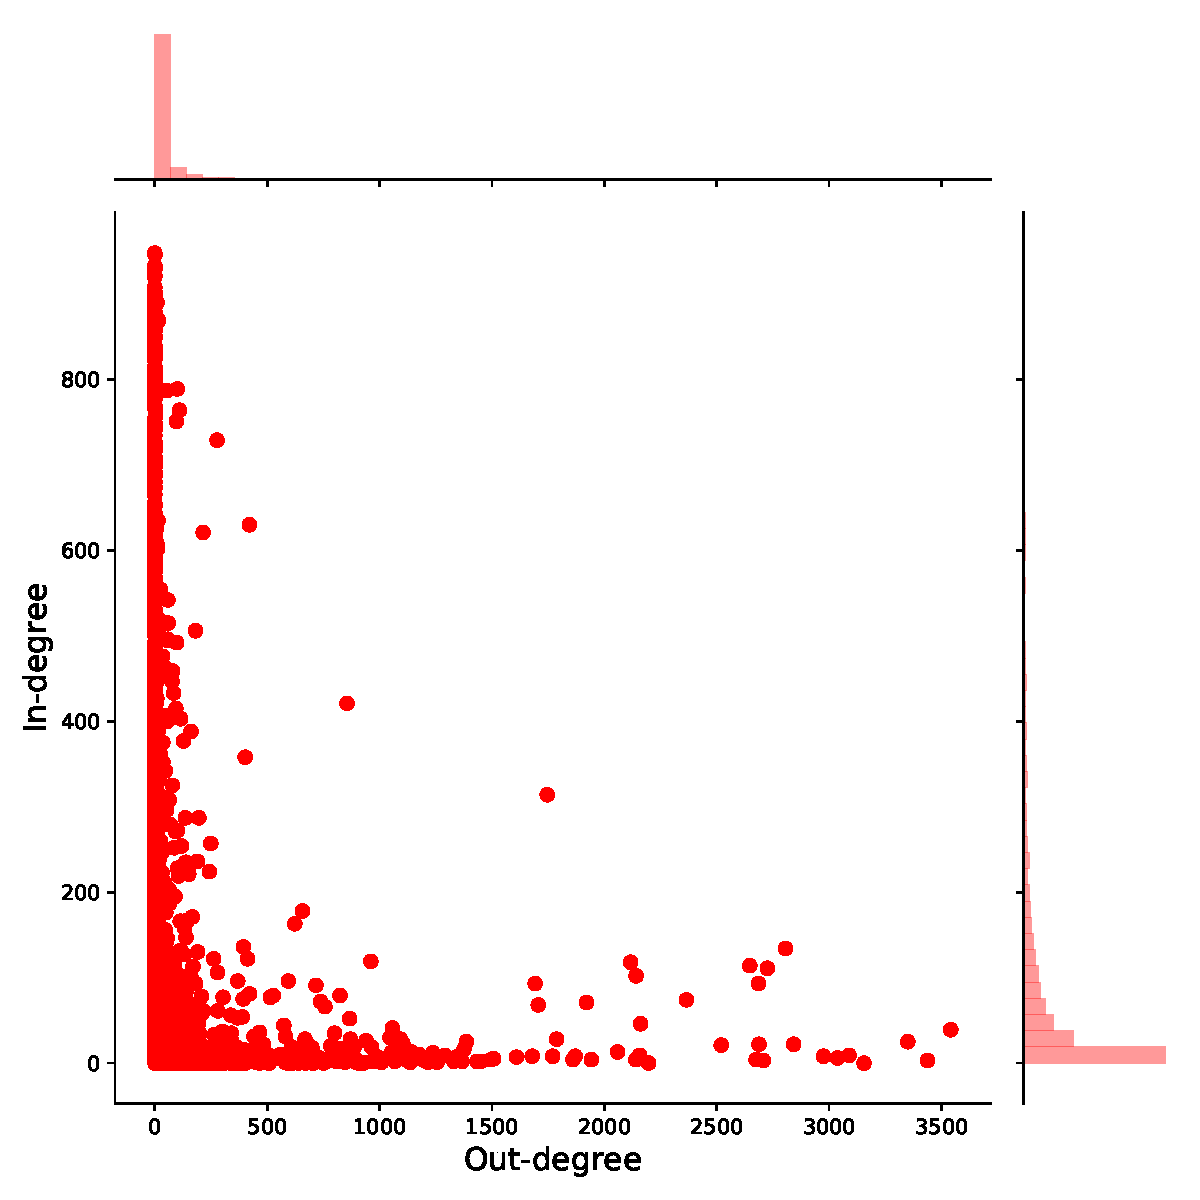
\includegraphics[width=.55\linewidth]{images/Aggregate/Degree/jointplot/attacks_jointplot_no_outliers}
	}
	\hfill
	\subfloat[Jointplot messaggi.]{%
	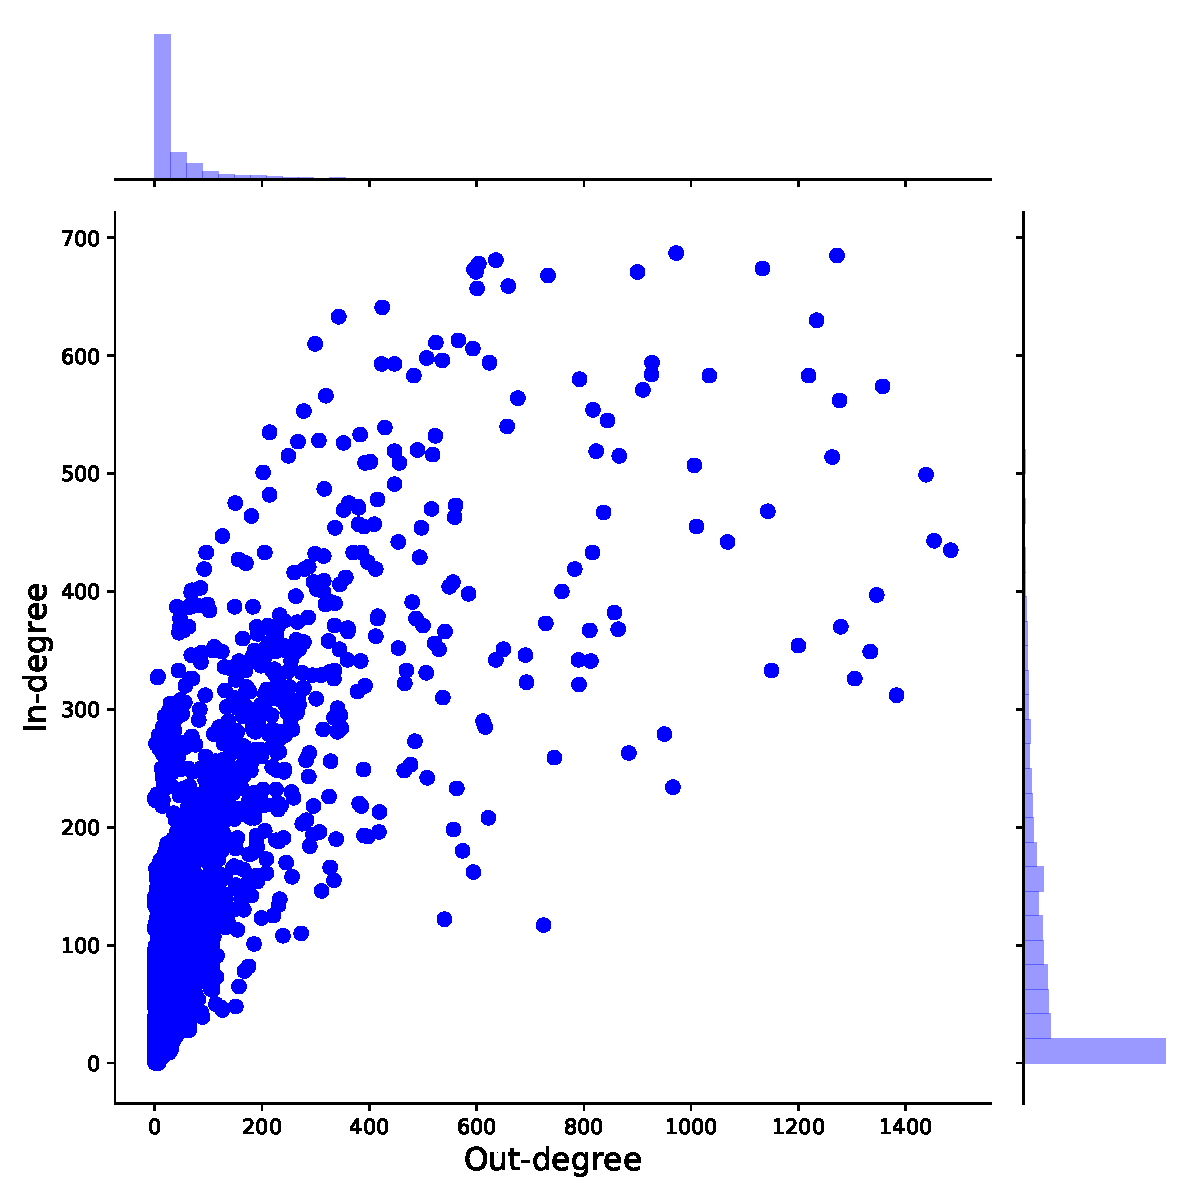
\includegraphics[width=.55\linewidth]{images/Aggregate/Degree/jointplot/messages_jointplot_no_outliers}
	}
	\hfill
	\subfloat[Jointplot trade.]{%
	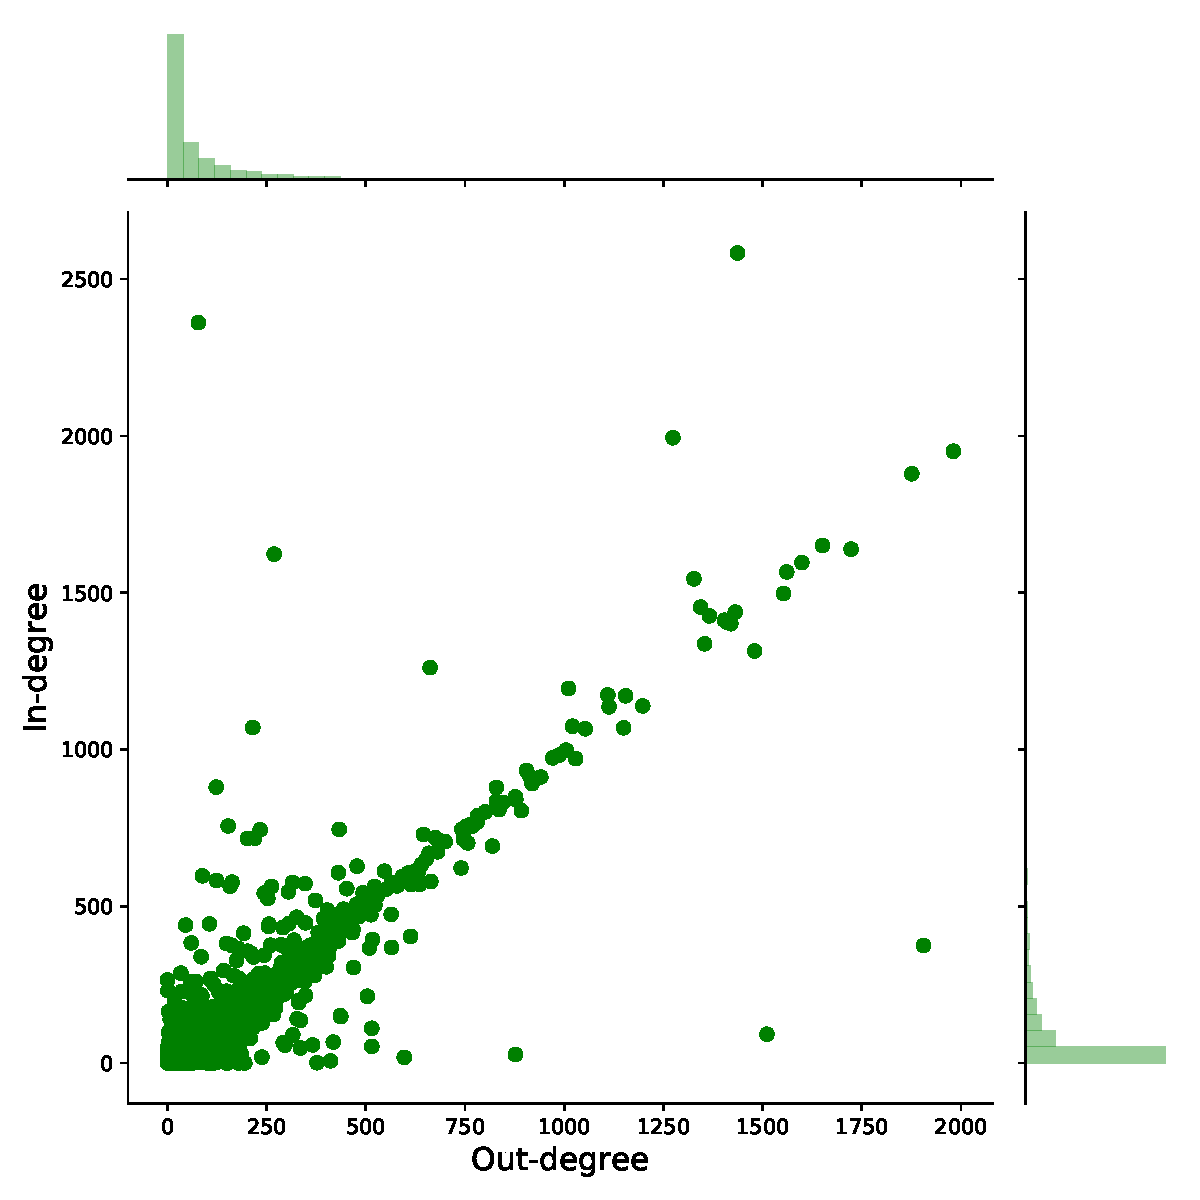
\includegraphics[width=.55\linewidth]{images/Aggregate/Degree/jointplot/trades_jointplot}
	}
	\caption{Jointplot che pongono in relazione in-degree e out-degree del layer specificato.}
	\label{fig:join_degree}
\end{figure}

In ultimo, sono stati generati i \textit{jointplot} che pongono in relazione gli out-degree di messaggi e attacchi o trade, rispettivamente in Figura \ref{subfig:joint_m_a} e \ref{subfig:joint_m_t}. Dal primo grafico si evince come numero di attacchi e numero di messaggi siano solitamente inversamente proporzionali, mentre non vi sembra essere una stretta relazione tra messaggi e scambi commerciali.
\begin{figure}
	\subfloat[Jointplot tra messaggi e attacchi.\label{subfig:joint_m_a}]{%
		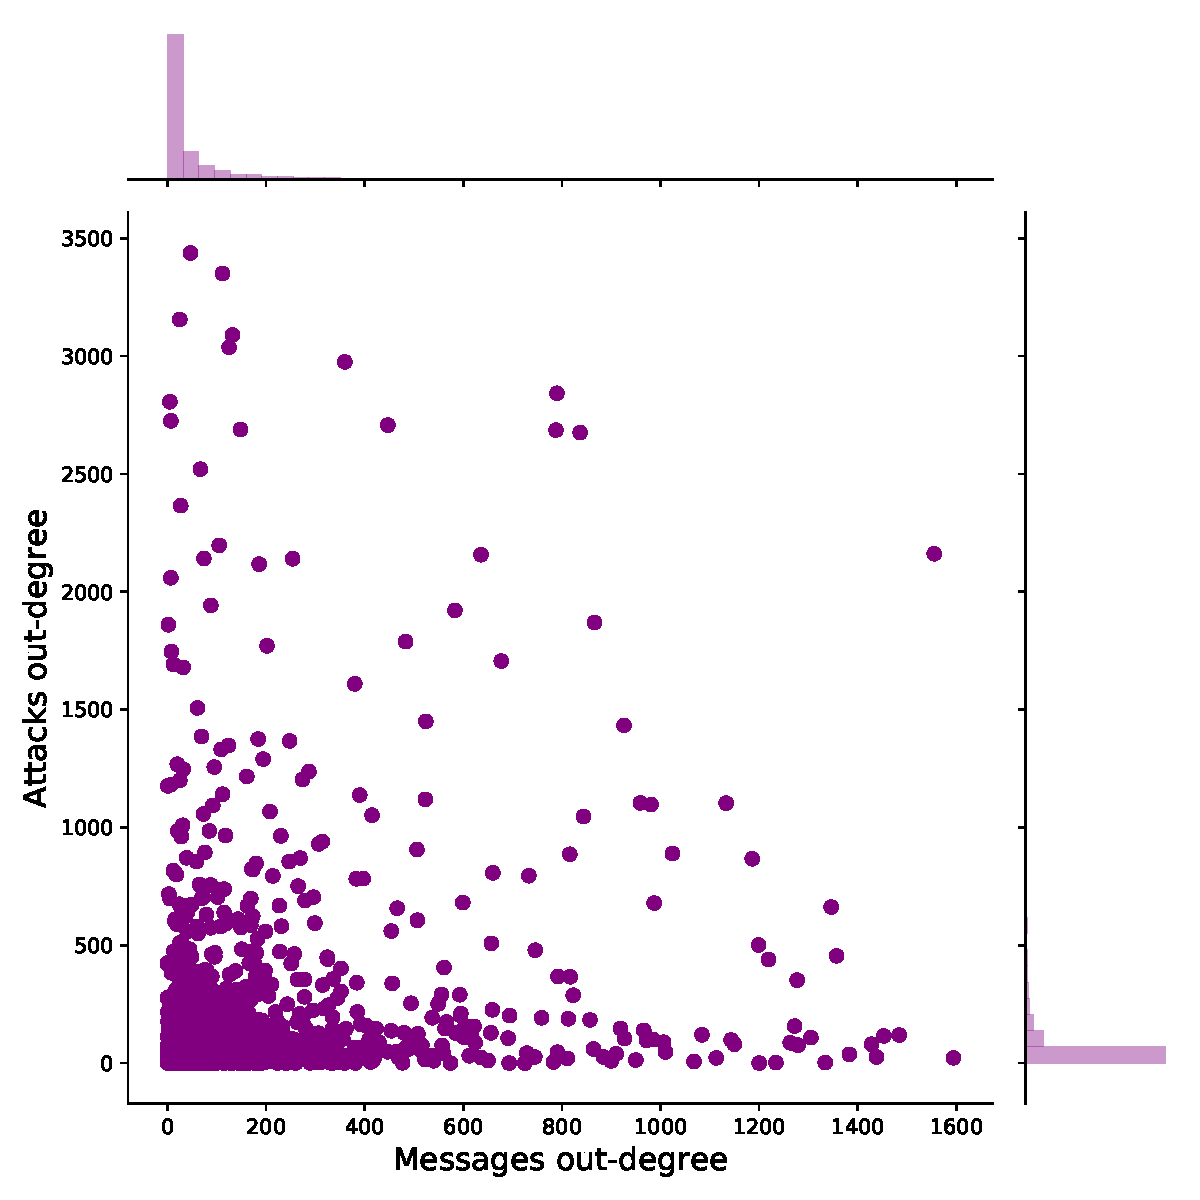
\includegraphics[width=.55\linewidth]{images/Aggregate/Degree/jointplot/messages_out-degree_vs_attacks_out-degree}
	}
	\hfill
	\subfloat[Jointplot tra messaggi e scambi.\label{subfig:joint_m_t}]{%
		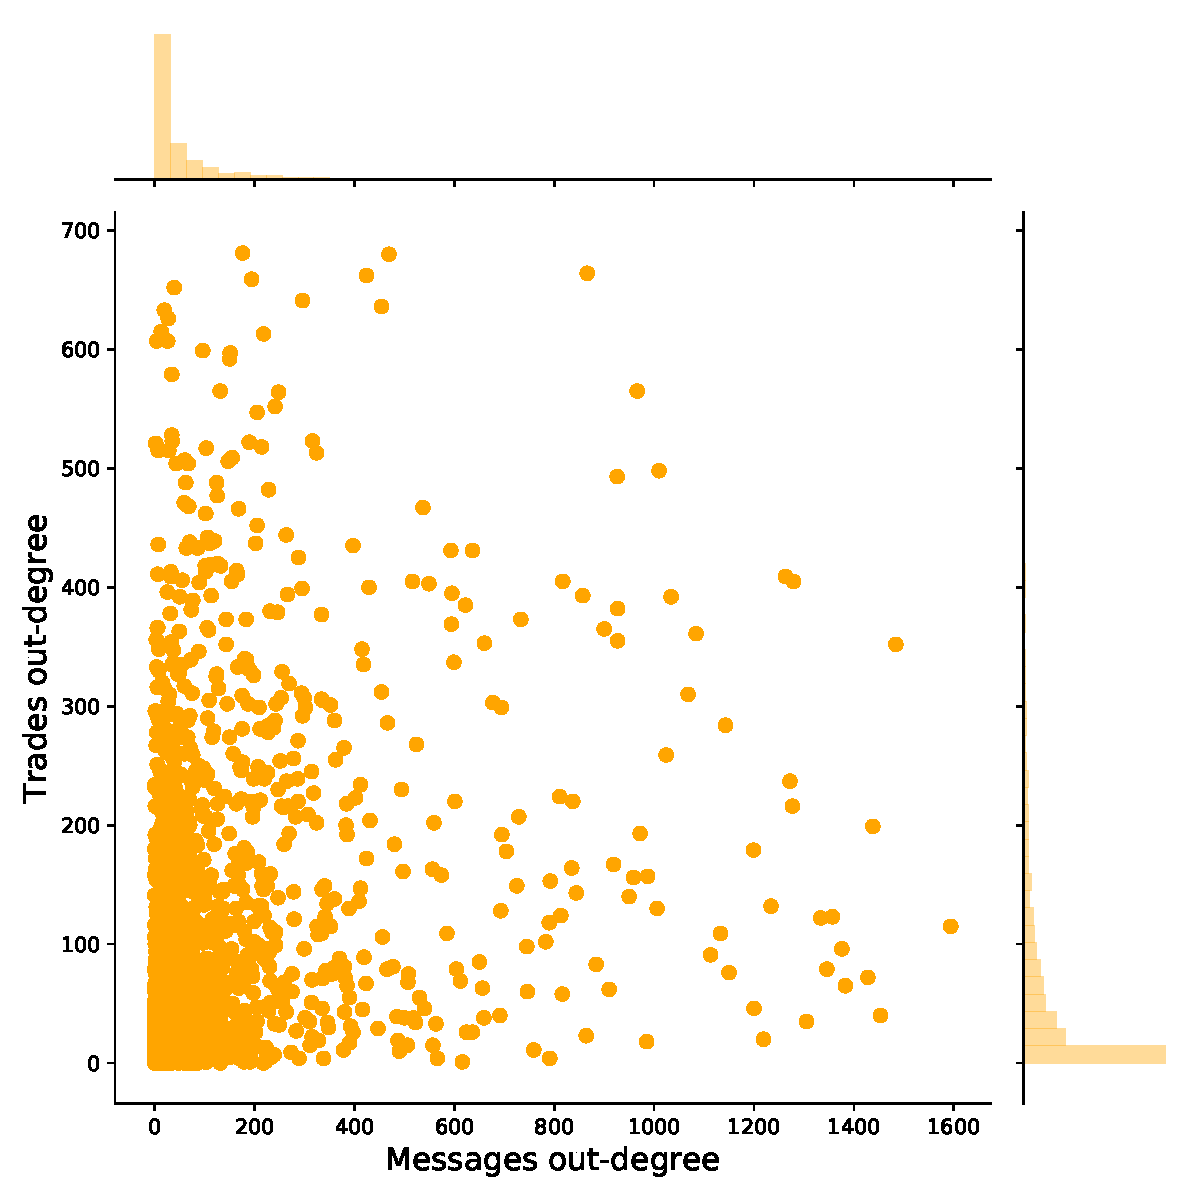
\includegraphics[width=.55\linewidth]{images/Aggregate/Degree/jointplot/messages_out-degree_vs_trades_out-degree}
	}
	\caption{Jointplot che pongono in relazione out-degree dei diversi layer.}
	\label{fig:join_mixed}
\end{figure}

\subsection{Misure di centralità}
\label{subsec:centrality}
Per quanto riguarda le misure di centralità, abbiamo deciso di concentrare i nostri approfondimenti esclusivamente sui layer di messaggi e scambi, in quanto sulla rete di attacchi il calcolo di queste misure risulta essere poco sensato (non vi è alcun flusso informativo).\\
Le misure analizzate per i due layer considerati sono:
\begin{itemize}
	\item Betweenness: misura che rappresenta il grado di informazione passante per un dato nodo. Un elevato valore indica un nodo centrale nel flusso informativo / commerciale, con una grande capacità di collegamento tra porzioni della rete.
	\item PageRank: calcola l'importanza di un nodo grazie al numero di archi entranti e al peso dei nodi che lo referenziano. Fornisce un'informazione pesata e più specifica rispetto al semplice grado in ingresso.
\end{itemize}

Per il layer dei messaggi, i grafici delle due misure analizzate, riportati in Figura \ref{fig:messages_centrality}, mostrano una predominanza del contatto diretto rispetto al passaggio di informazione secondo una scala di gradi. Un distribuzione dei valori di betweenness concentrata in valori molto bassi, indica la presenza di molti collegamenti alternativi tra due nodi: non si presenta quindi la situazione di un passaggio "forzato" per un determinato nodo. PageRank mostra un andamento simile, non individuando chiaramente dei nodi predominanti sugli altri. Si noti che dal dataset sono stati rimossi tutti i messaggi di \textit{broadcast}, ovvero le comunicazioni inviate dai gestori delle alleanze a tutti i membri di essa: questo ha certamente influenzato una compressione di valori delle due misure precedentemente analizzate.\\ 
\begin{figure}
	\subfloat[Centralità Betweenness.]{%
		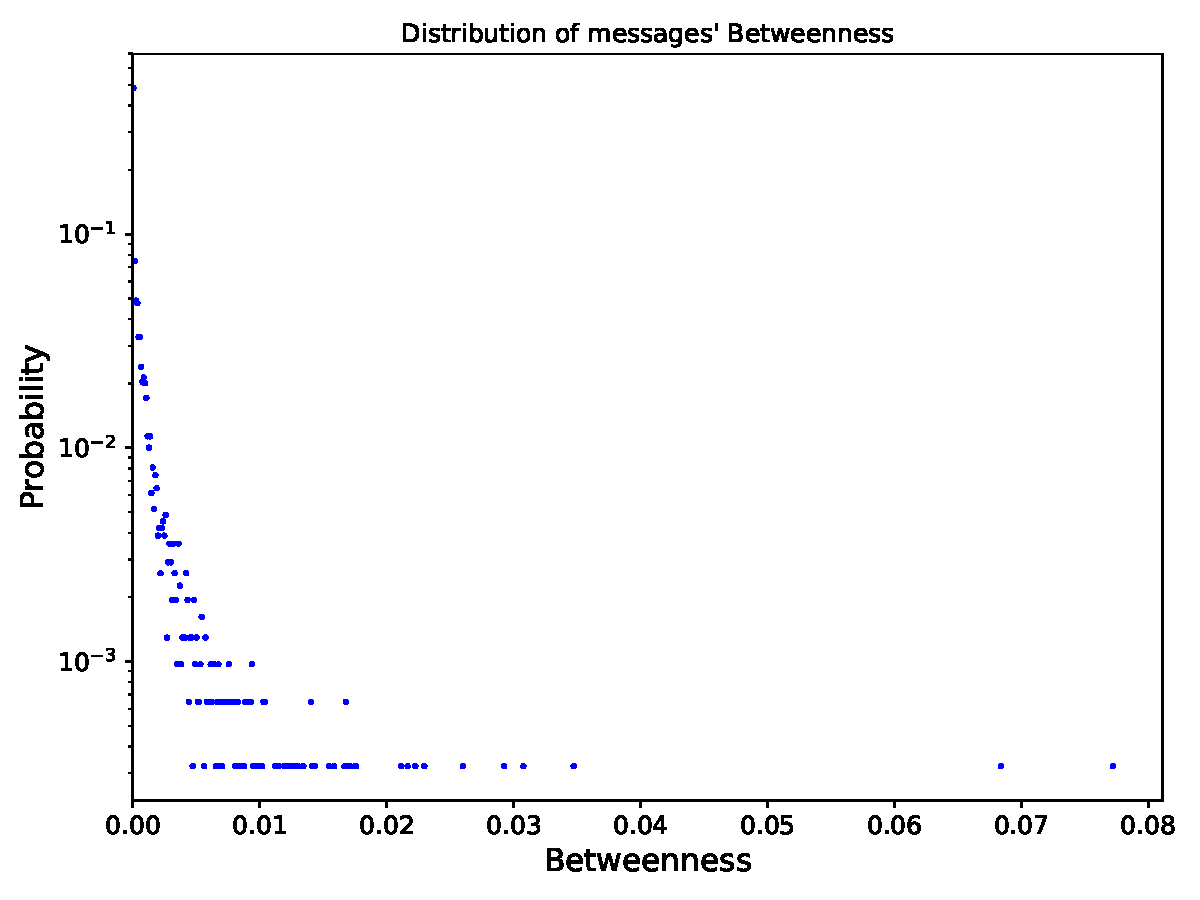
\includegraphics[width=.55\linewidth]{images/Aggregate/Centrality/messages_betweenness}
	}
	\hfill
	\subfloat[Centralità Pagerank.]{%
		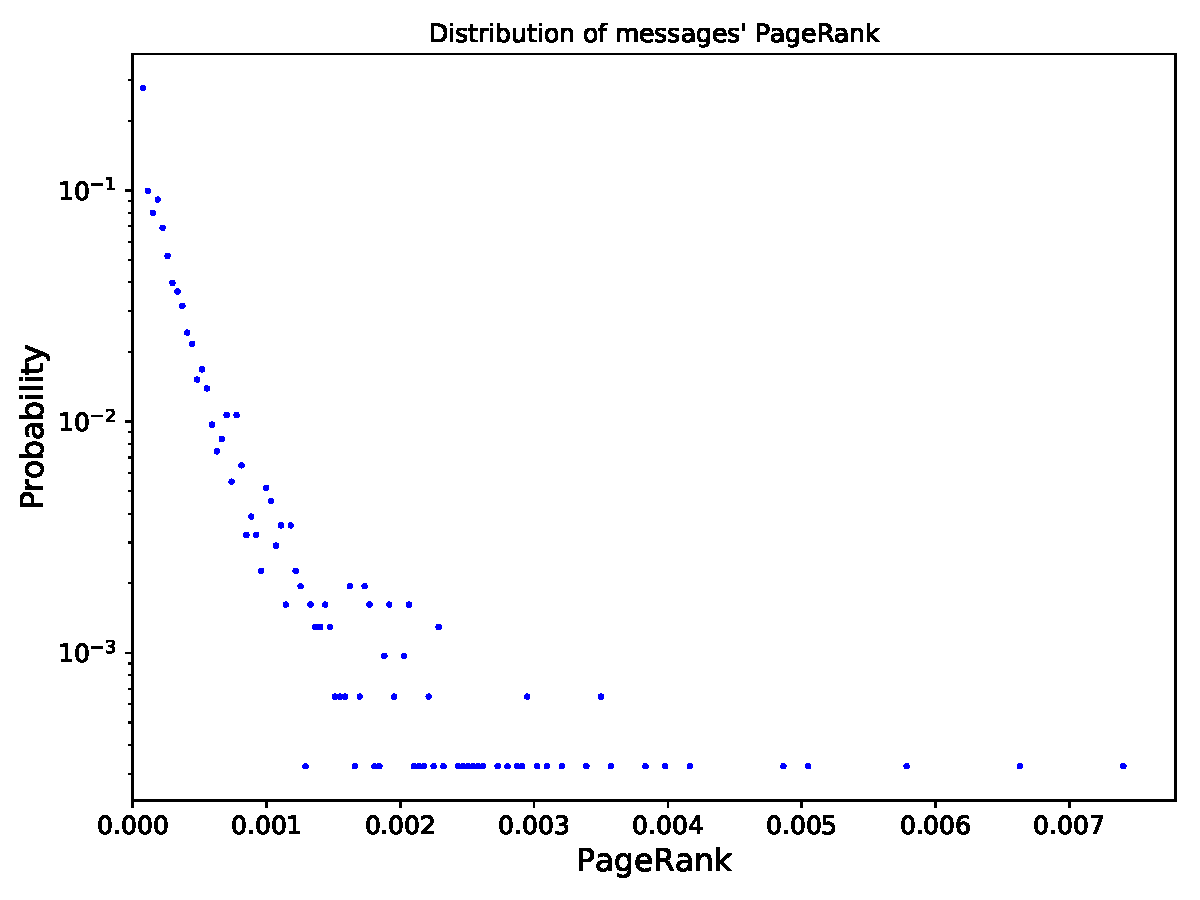
\includegraphics[width=.55\linewidth]{images/Aggregate/Centrality/messages_PageRank}
	}
	\caption{Grafici delle misure di centralità calcolate sul layer dei messaggi.}
	\label{fig:messages_centrality}
\end{figure}
Lo stesso comportamento è mostrato dall'analisi del grafo degli scambi (in Figura \ref{fig:trades_centrality}), con valori della betweenness ancora più compressi rispetto ai messaggi. Ciò è probabilmente dovuto all'assenza di figure di passaggio delle merci: non vi è un "mercante" che acquista beni da un insieme di giocatori per poi rivendere ad altri, ma i giocatori sono liberi di commerciare direttamente tra loro.
\begin{figure}
	\subfloat[Centralità Betweenness.]{%
		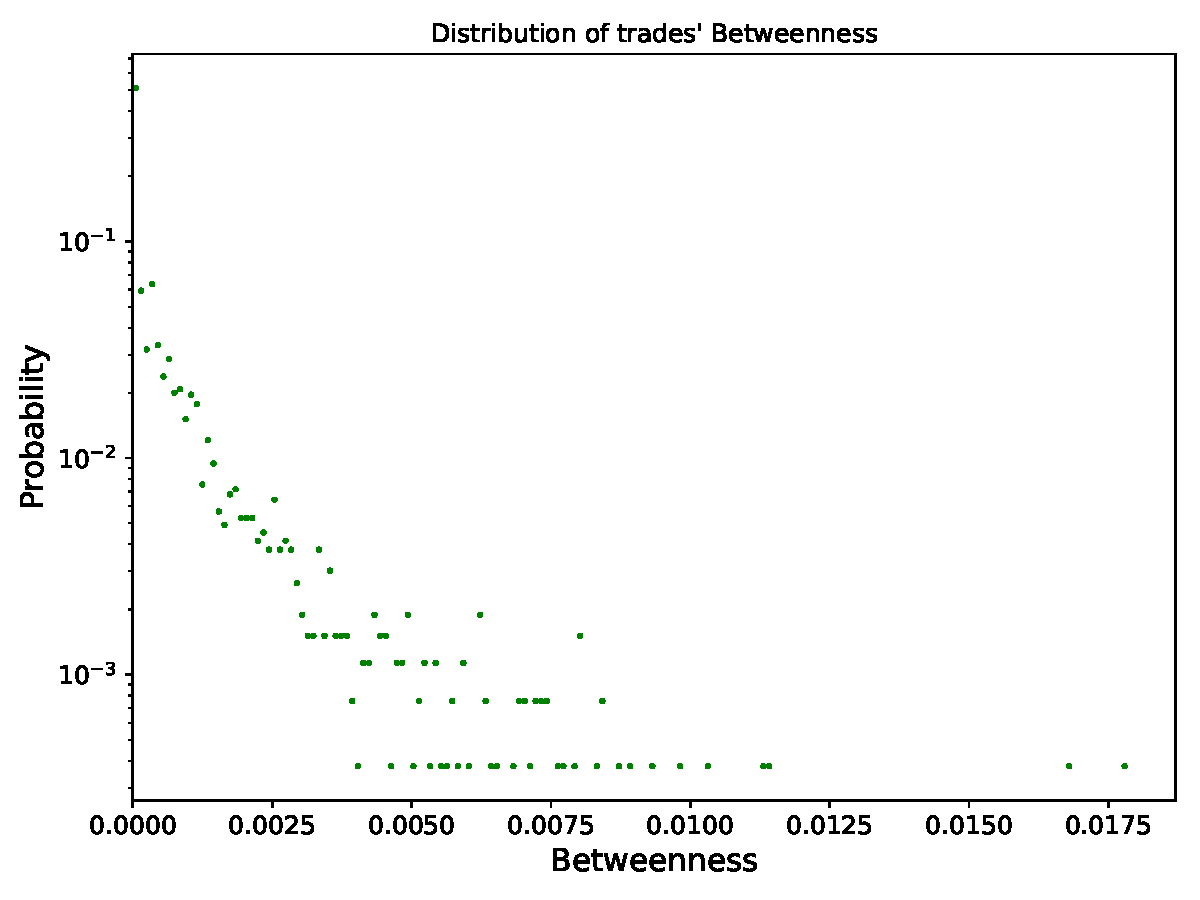
\includegraphics[width=.55\linewidth]{images/Aggregate/Centrality/trades_betweenness}
	}
	\hfill
	\subfloat[Centralità Pagerank.]{%
		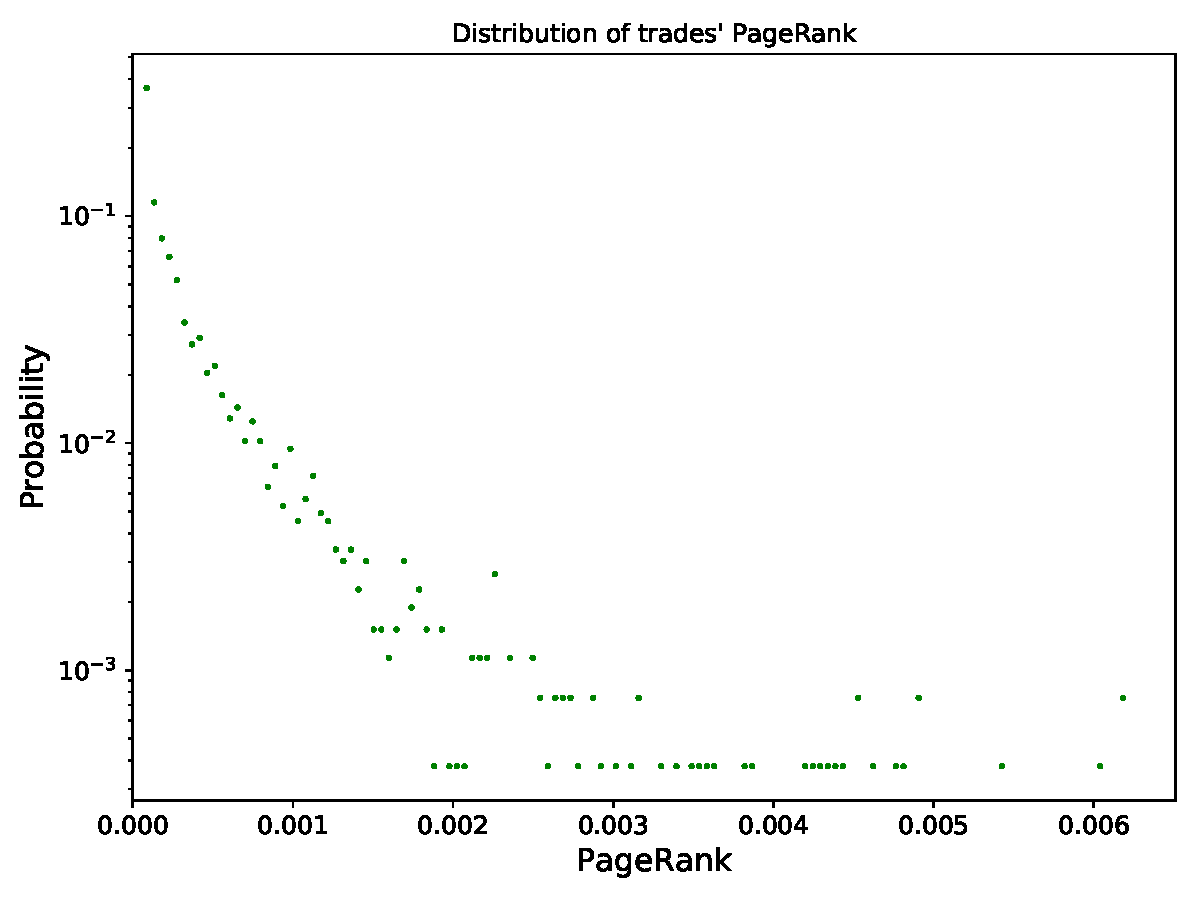
\includegraphics[width=.55\linewidth]{images/Aggregate/Centrality/trades_PageRank}
	}
	\caption{Grafici delle misure di centralità calcolate sul layer dei trade.}
	\label{fig:trades_centrality}
\end{figure}

Abbiamo infine generato i jointplot delle due misure analizzate, per individuare possibili correlazioni tra i valori delle due. I risultati, riportati in Figura \ref{fig:joint_centrality}, mostrano come la maggioranza dei nodi si concentri nei pressi dell'origine degli assi, a cui corrispondono bassi valori di entrambe le misure. Sono apprezzabili diversi outliers in entrambi i grafici, che mostrano \todo{indagare su questi outliers}
\begin{figure}
	\subfloat[Jointplot messaggi.]{%
		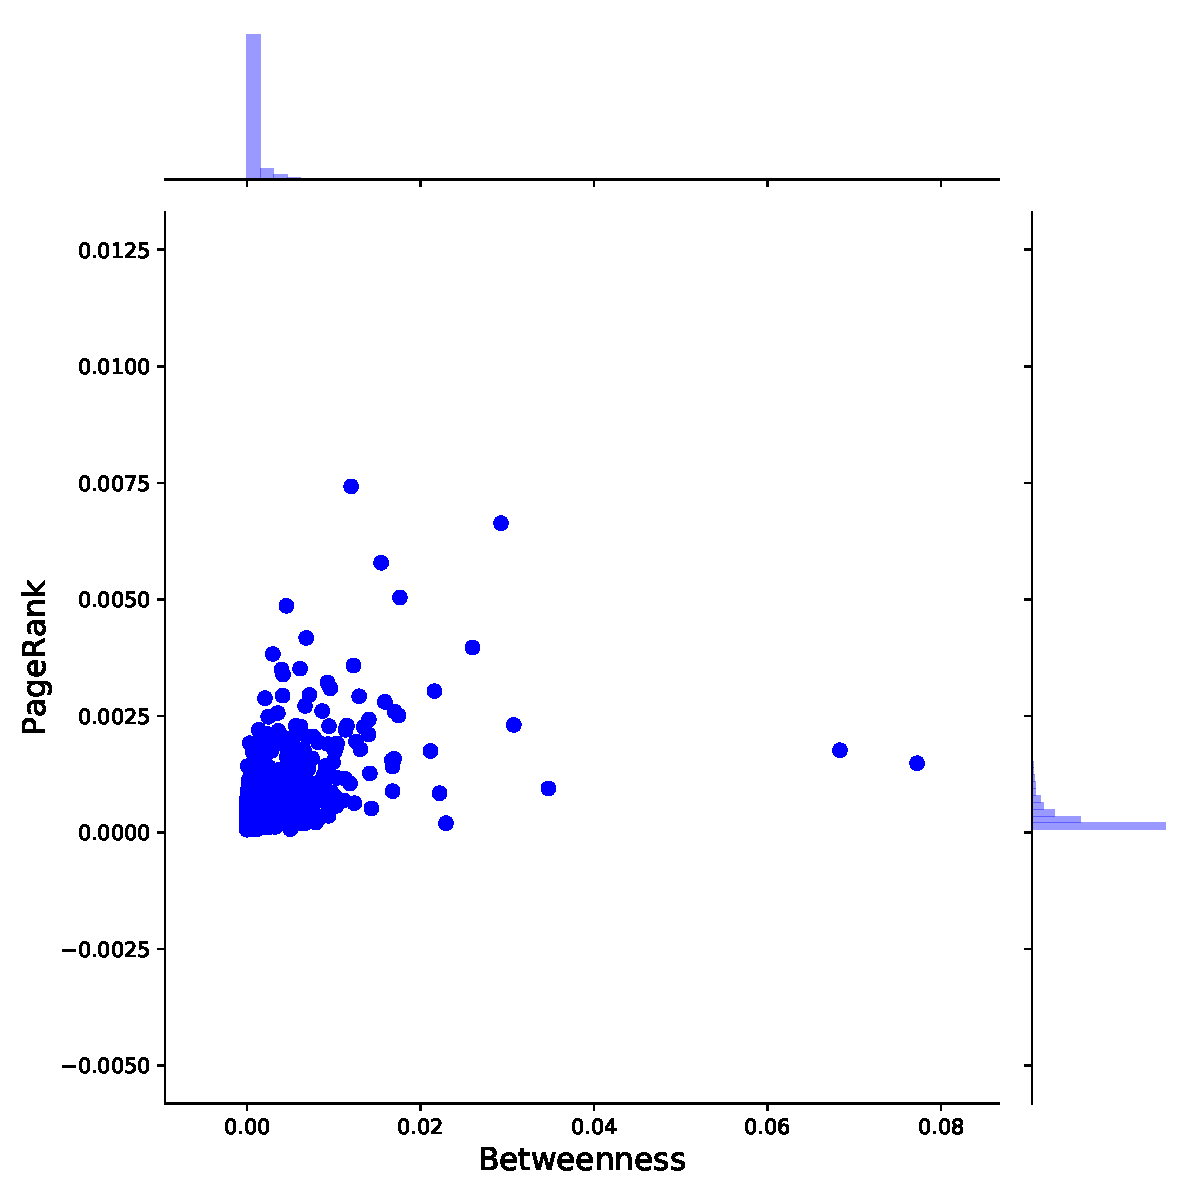
\includegraphics[width=.55\linewidth]{images/Aggregate/Centrality/messages_jointplot}
	}
	\hfill
	\subfloat[Jointplot trade.]{%
		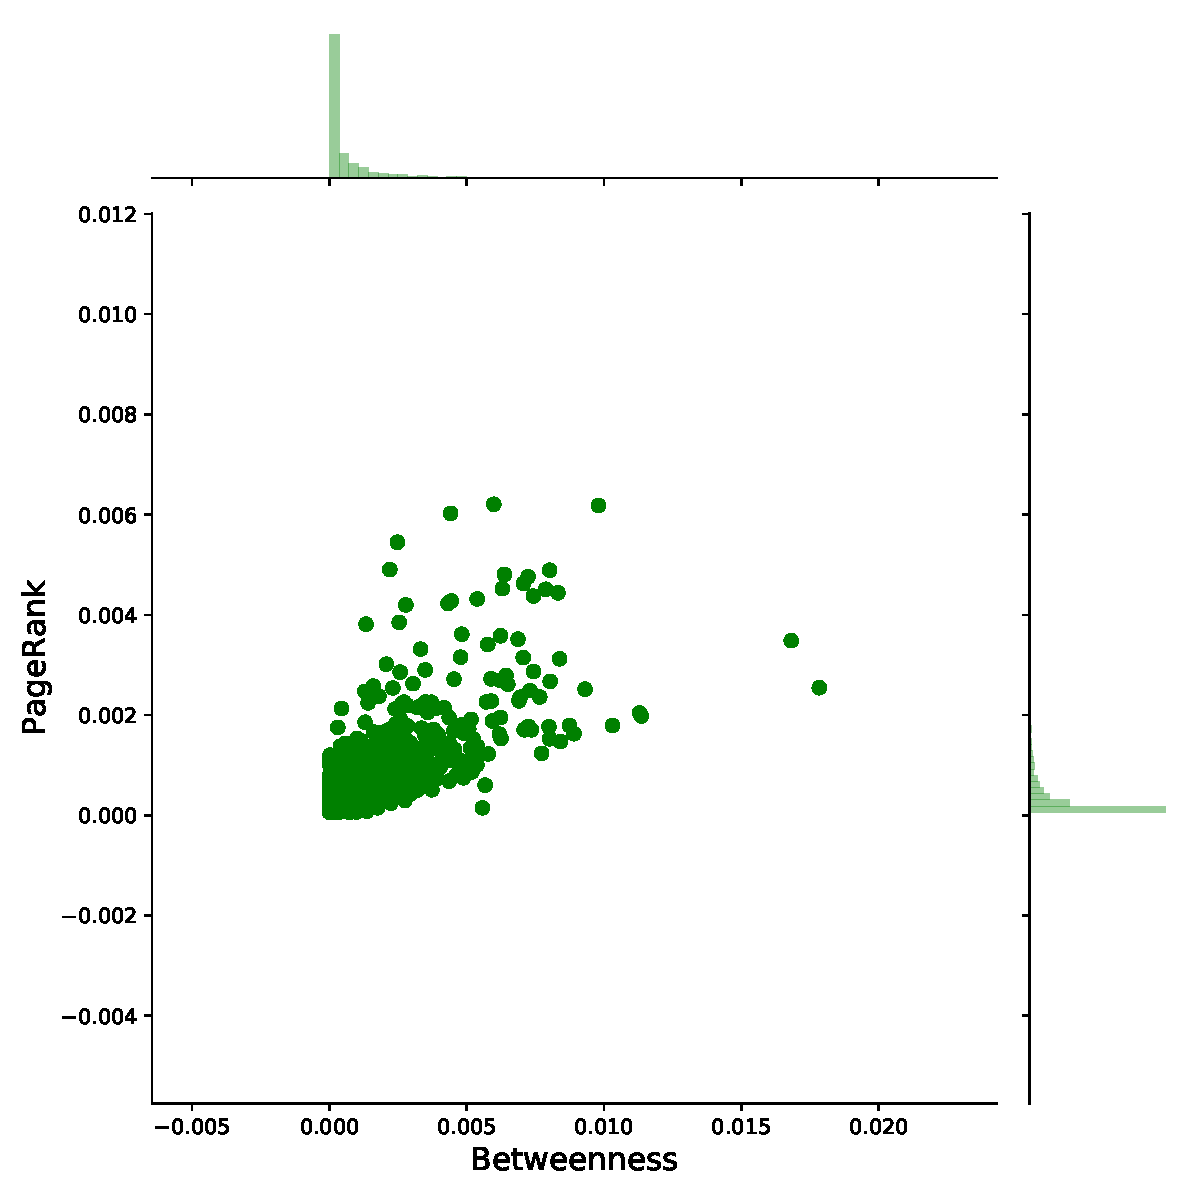
\includegraphics[width=.55\linewidth]{images/Aggregate/Centrality/trades_jointplot}
	}
	\caption{Jointplot delle misure di centralità calcolate rispettivamente sui messaggi e sugli scambi.}
	\label{fig:joint_centrality}
\end{figure}

\newpage
\subsection{Coefficiente di clustering medio}
Un'ulteriore misura analizzata è stata il coefficiente medio di clustering, ovvero la misura della tendenza di un nodo a formare un cricca (i.e. grafo completo). Questo comportamento è solito rilevarsi nelle reti sociali, dove i nodi tendono a formare delle community dense e coese rispetto al resto del grafo. Essendo questa una misura media, bisogna considerare il fatto che la maggior parte dei nodi non facciano parte di alcuna community, e questo influenzi molto il valore medio ottenuto: useremo i risultati di questa analisi come metro di paragone per i successivi studi sulle alleanze. 
I risultati ottenuti sono riportati in Figura \ref{fig:clustering}: vediamo come nel layer dei messaggi, che possiamo considerare una rete sociale, i valori medi sono decisamente maggiori rispetto alla rete degli scambi, dove i vicini di un nodo non necessariamente sono soliti commerciare tra loro. Ci possiamo altresì aspettare che i nodi del vicinato di x siano più propensi a conoscersi e a comunicare tra loro.
\ref{fig:messages_centrality}, mostrano 
\begin{figure}
	\subfloat[Coefficiente di clustering medio per i messaggi.]{%
		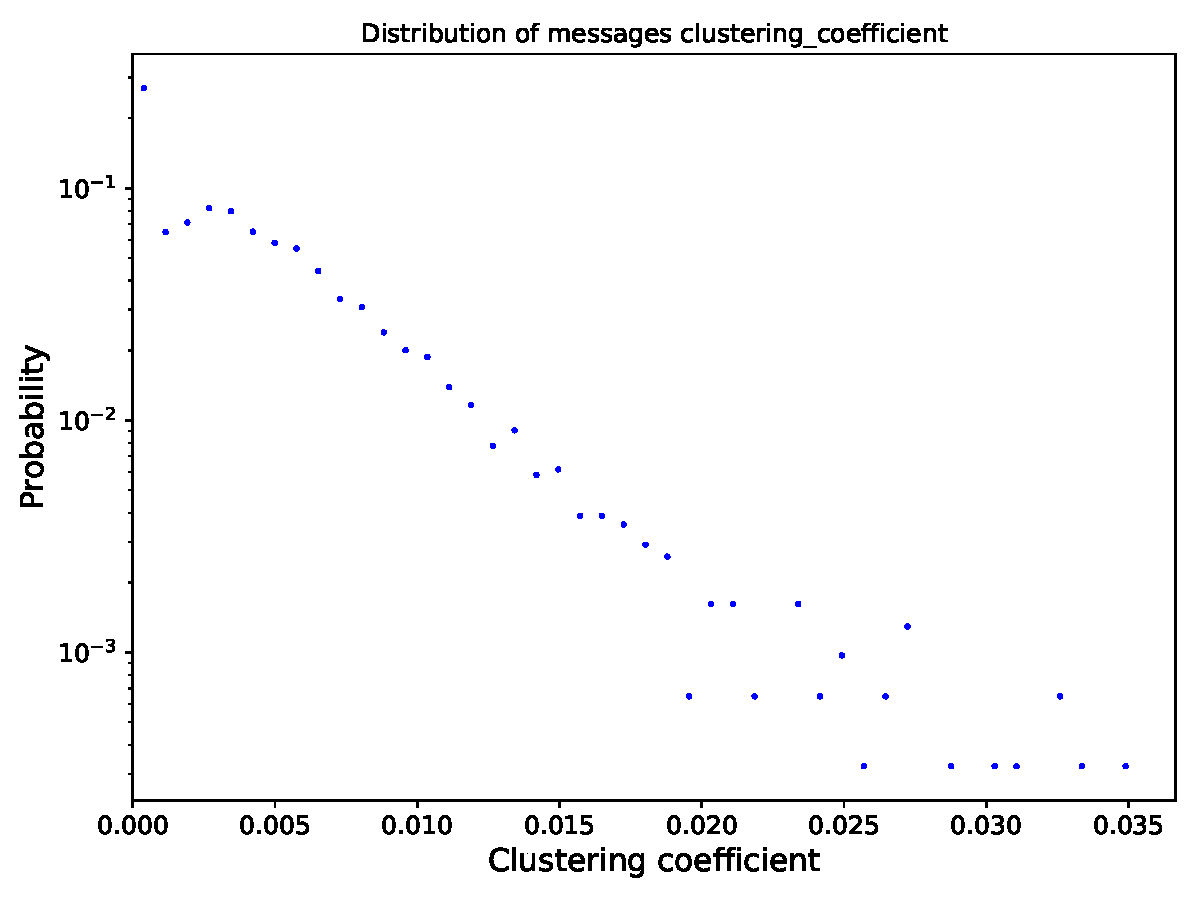
\includegraphics[width=.55\linewidth]{images/Aggregate/Clustering/messages}
	}
	\hfill
	\subfloat[Coefficiente di clustering medio per i trade.]{%
		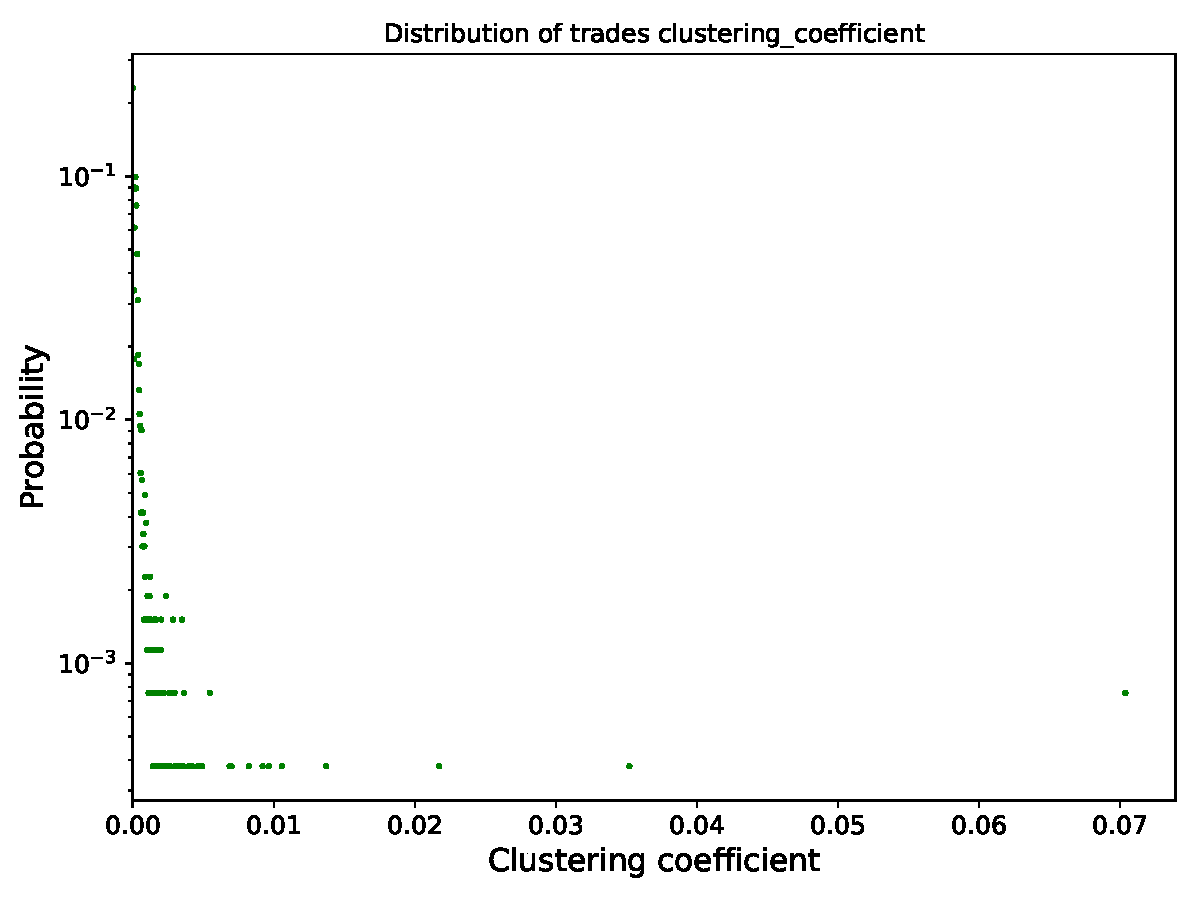
\includegraphics[width=.55\linewidth]{images/Aggregate/Clustering/trades}
	}
	\caption{Grafici delle misure di centralità calcolate sul layer dei messaggi.}
	\label{fig:clustering}
\end{figure}

\newpage 
\section{Analisi delle attività}
Un'ulteriore analisi condotta sul dataset è stata la distribuzione giornaliera di attività durante il periodo analizzato: ci siamo chiesti se fosse possibile delineare una qualche relazione tra i dati disponibili, in particolare tra numero di giocatori ed attività.\\
Il numero di giocatori attivi sul server in almeno uno dei tre layer è rappresentato in Figura \ref{fig:playereachday}, dove si può notare un drastico calo al giorno 5.
\begin{figure}
	\centering
	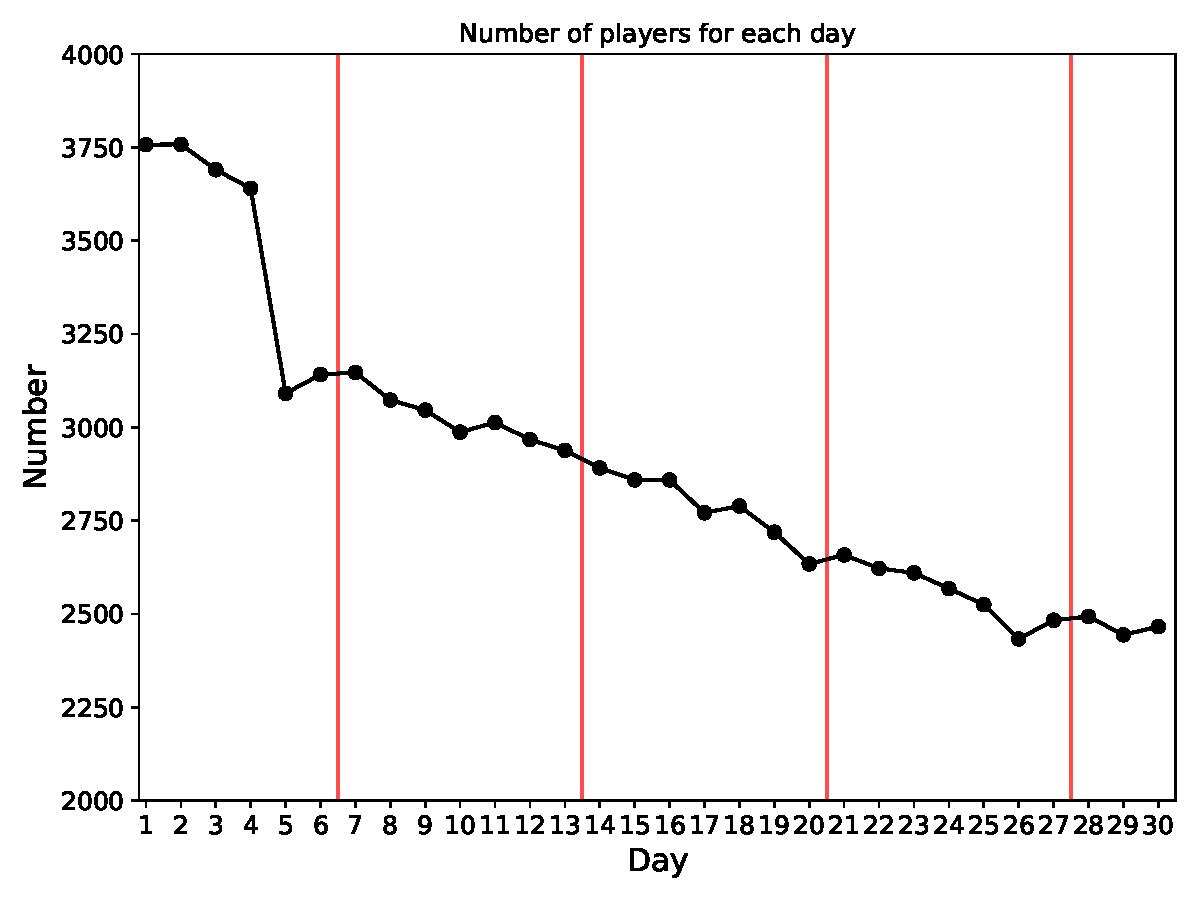
\includegraphics[width=0.8\linewidth]{images/Activity/player_each_day}
	\caption{Numero di giocatori attivi in un dato giorno. rappresentano l'inizio di una nuova settimana.}
	\label{fig:playereachday}
\end{figure}
Come mostrato in Figura \ref{fig:activity_each_day}, complessivamente il numero di azioni eseguite dai giocatori decresce lungo il periodo analizzato, con picchi durante i week-end e le festività. 
\begin{figure}
	\subfloat[Numero di archi presenti nei vari layer ad un dato giorno.]{%
		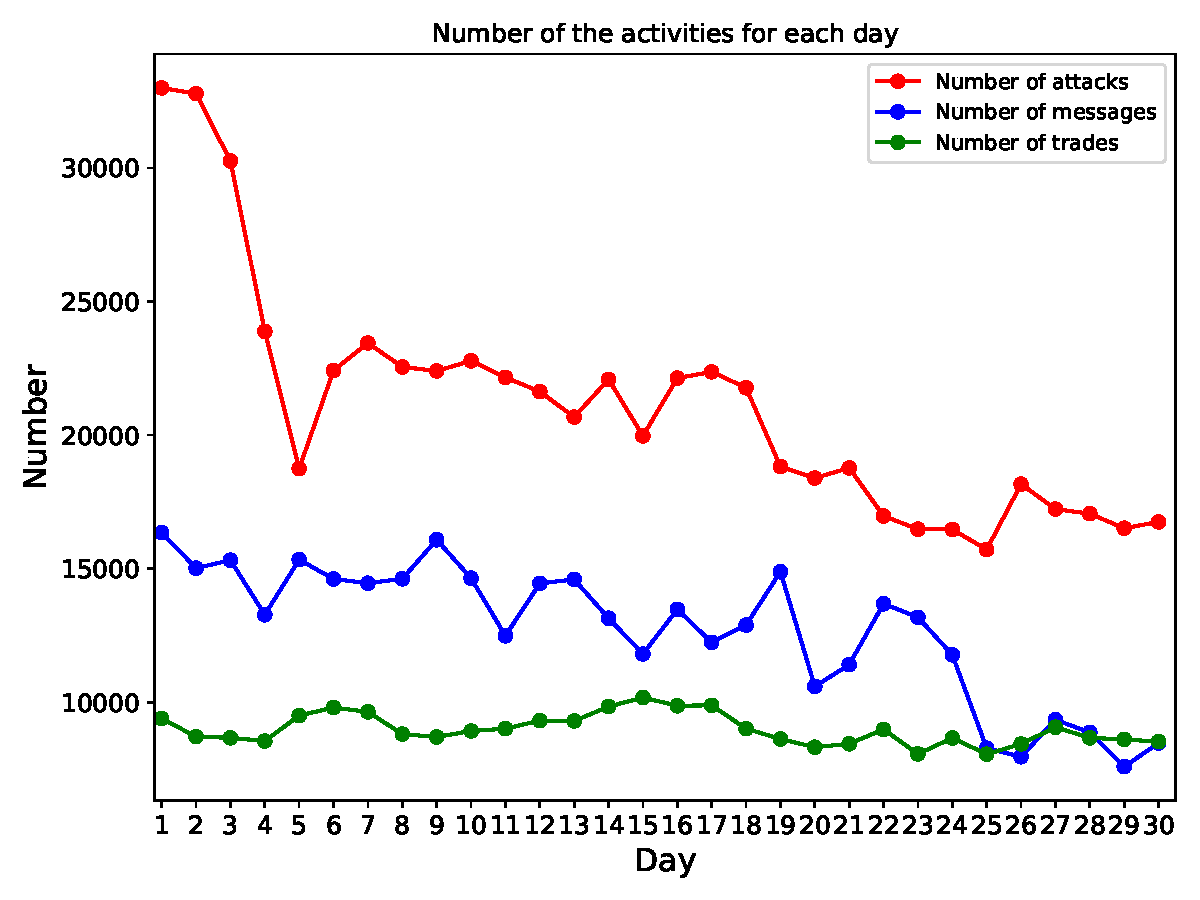
\includegraphics[width=.45\linewidth]{images/Activity/n_each_activity_each_day}
	}
	\hfill
	\subfloat[Somma del numero di archi presenti nei tre layer ad un dato giorno.]{%
		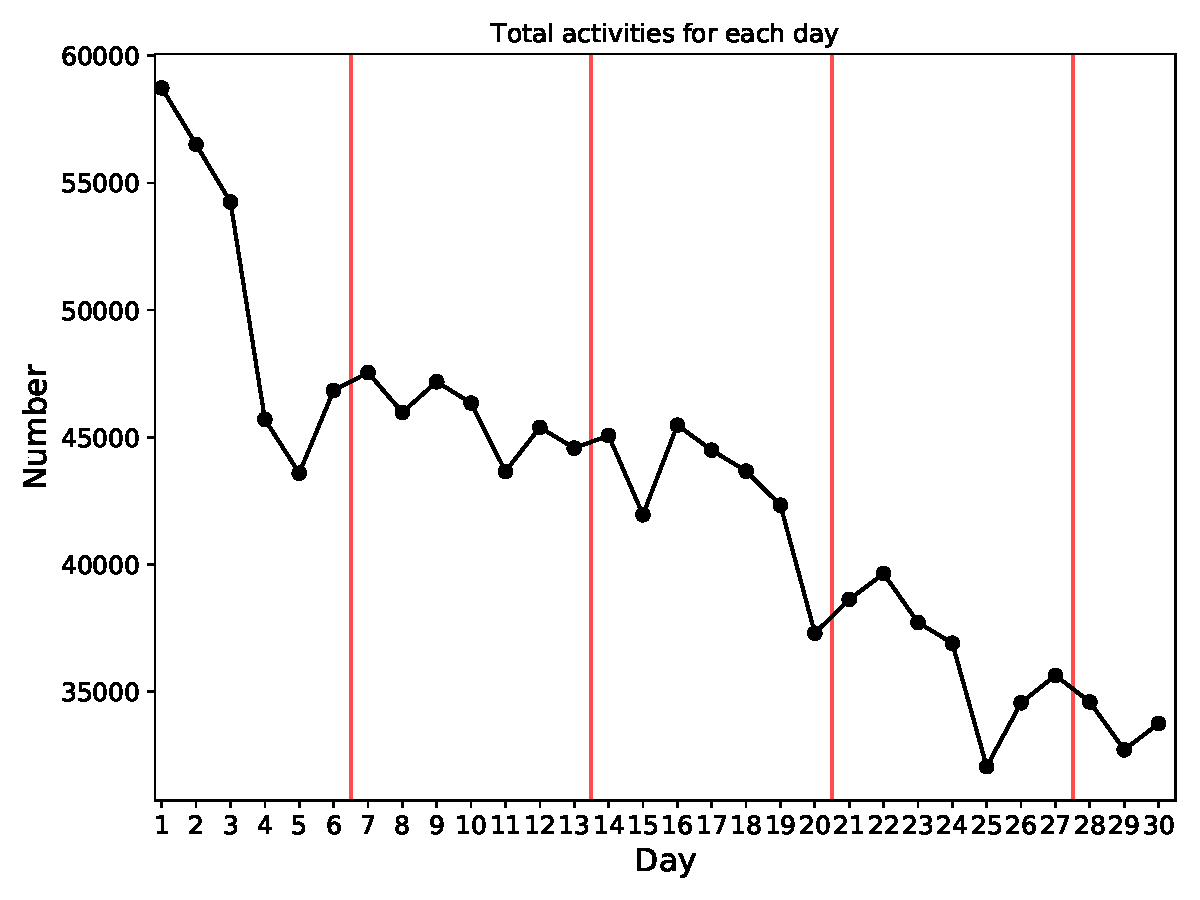
\includegraphics[width=.45\linewidth]{images/Activity/total_activities_each_day}
	}
	\caption{Le linee rosse verticali nel grafico di destra rappresentano l'inizio di una nuova settimana. Si può apprezzare un andamento complessivamente decrescente, soprattutto in corrispondenza del week-end e di festività.}
	\label{fig:activity_each_day}
\end{figure}
In Figura \ref{fig:activity_players} è possibile osservare la relazione tra numero di giocatori e attività eseguite. Come ci aspettavamo, l'andamento delle due curve risulta essere appaiato, e mantiene il trend decrescente individuato dai grafici in Figura \ref{fig:activity_each_day} e \ref{fig:playereachday}.
\begin{figure}
	\subfloat[Numero di giocatori che hanno effettuato almeno un'azione nel layer specificato ad un dato giorno.]{%
		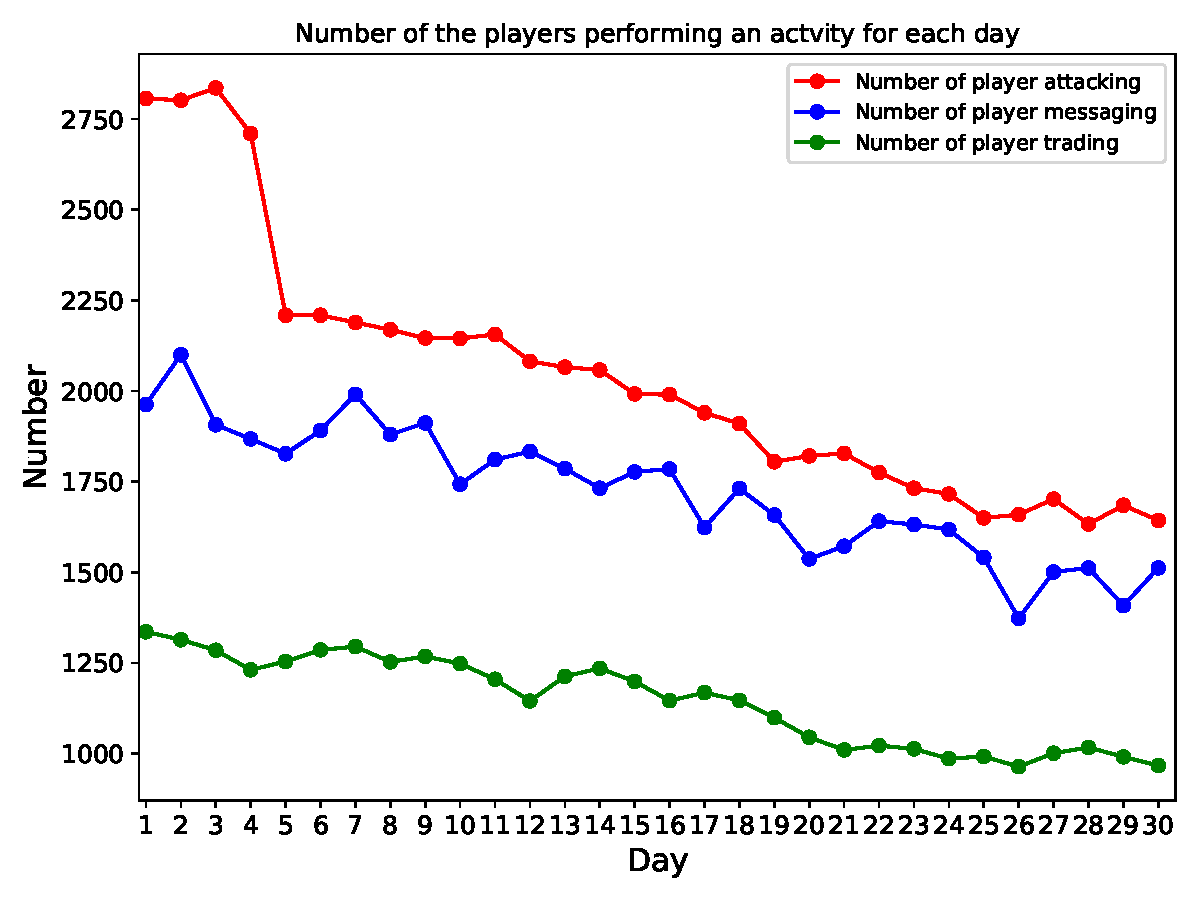
\includegraphics[width=.45\linewidth]{images/Activity/player_each_activity_each_day}
	}
	\hfill
	\subfloat[Andamento nei 30 giorni del numero di giocatori e delle attività totali.]{%
		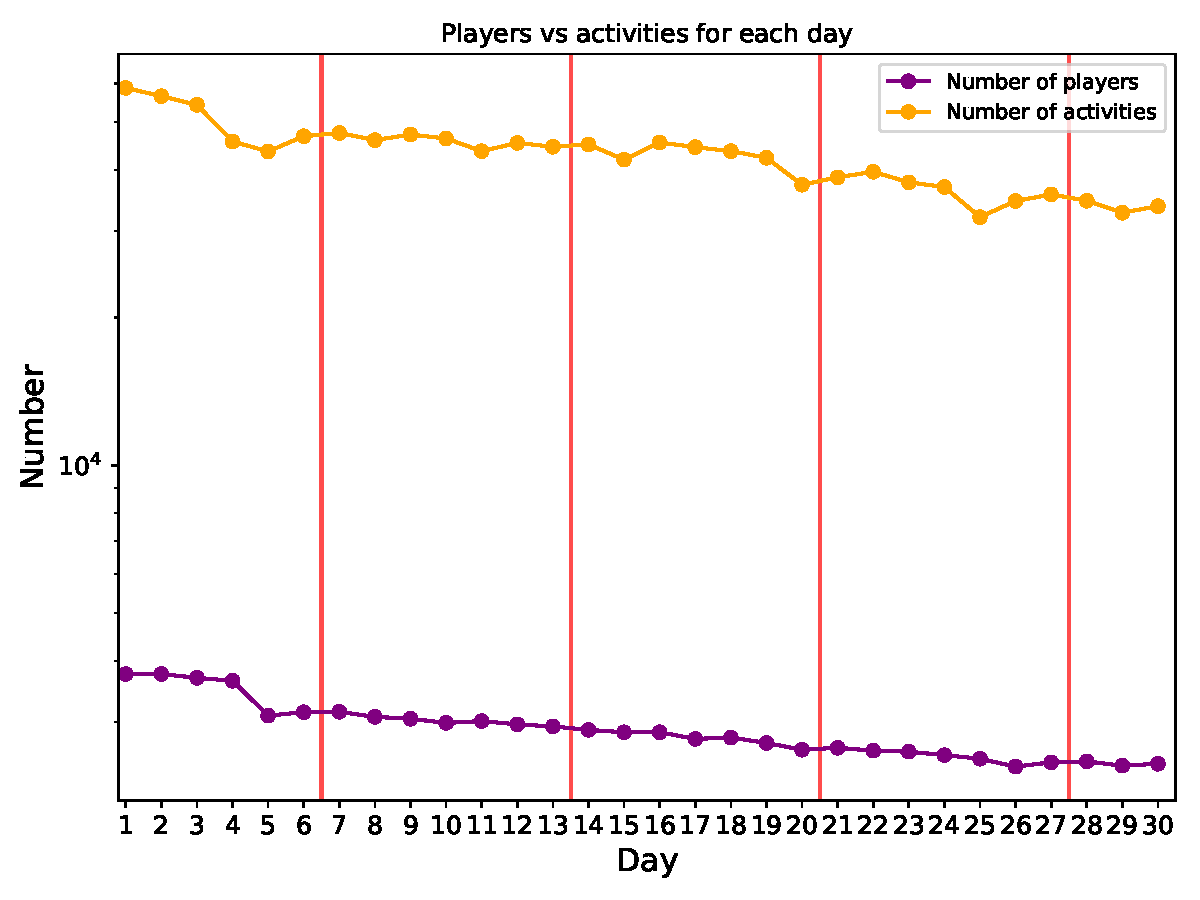
\includegraphics[width=.45\linewidth]{images/Activity/players_vs_activities_each_day}
	}
	\caption{L'andamento conferma il trend decrescente evidenziato anche in precedenza.}
	\label{fig:activity_players}
\end{figure}

In ultima battuta, abbiamo analizzato quali fossero gli orari dove si concentrasse il maggior numero di attività: in Figura \ref{fig:activity_players} sono riportati i nostri risultati. Notiamo come la maggioranza delle azioni sia eseguita tra le ore 14 e le 22, con un picco introno alle ore 18. L'andamento degli attacchi risulta essere più "liscio", probabilmente per l'elevata attività mattutina dovuta al tentativo di appropriarsi delle risorse accumulate nella notte dagli altri villaggi.\\
\begin{figure}
	\subfloat[Numero di attività per layer effettuate nei 30 giorni in una specifica fascia oraria.]{%
		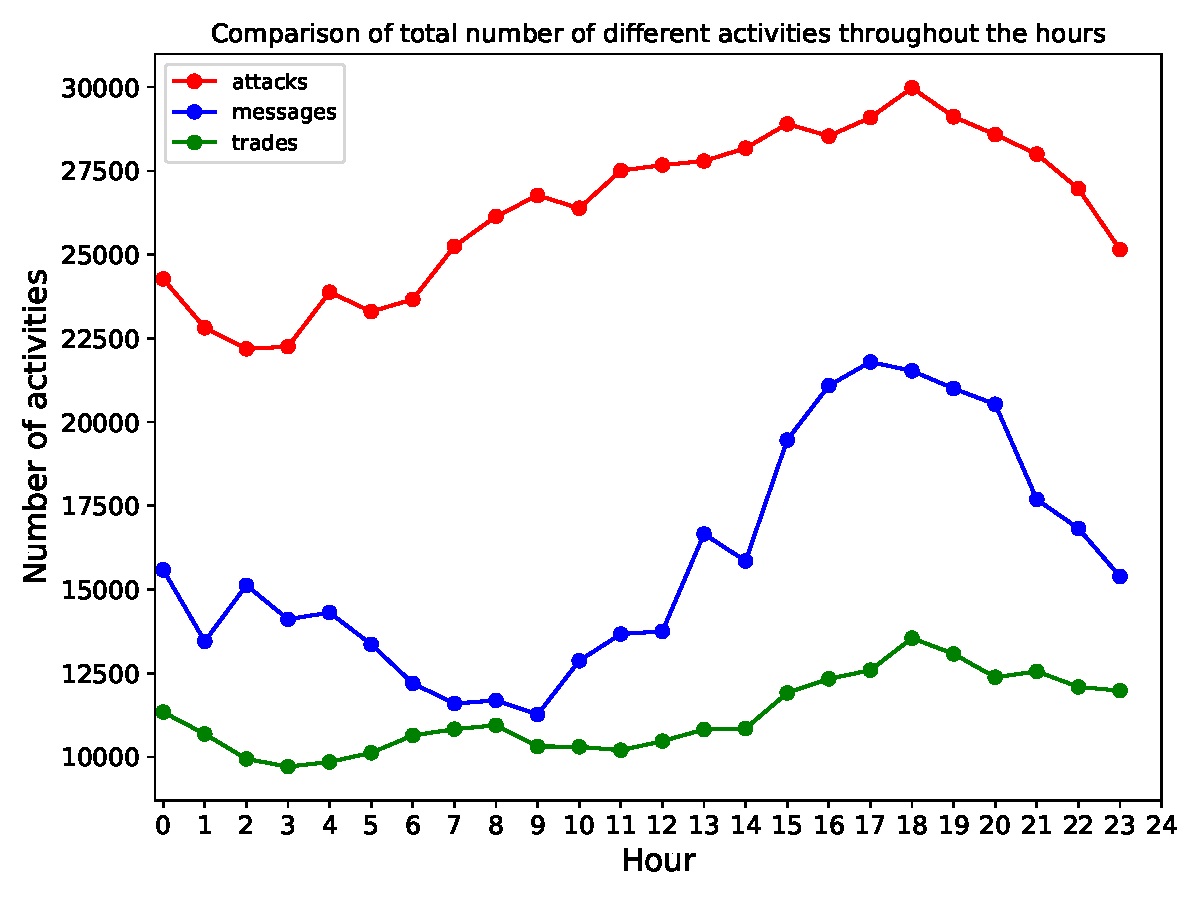
\includegraphics[width=.45\linewidth]{images/Activity/different_over_hours}
	}
	\hfill
	\subfloat[Numero di attività complessive per fascia oraria.]{%
		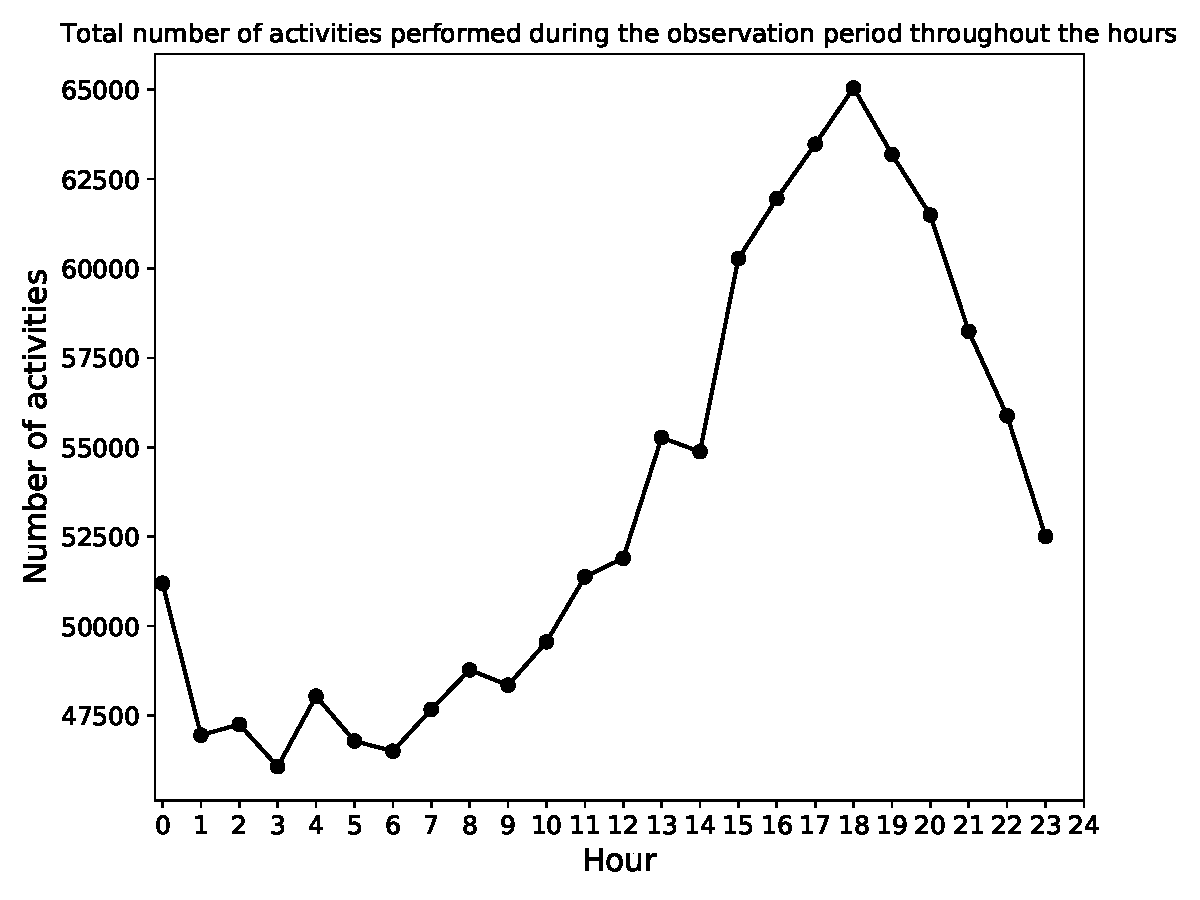
\includegraphics[width=.45\linewidth]{images/Activity/total_over_hours}
	}
	\caption{Attività sul server divisa per fascia oraria. Andamento crescente dalle ore 6 alle 18, poi decrescente fino alle 23}
	\label{fig:activity_players}
\end{figure}


\section{Ricerca di comportamenti sospetti}
Travian sostiene di aver implementato nel suo strumento di chat un metodo per impedire lo spam di messaggi verso altri utenti: se viene rilevata un grande numero di messaggi in uscita con il medesimo timestamp, il sistema blocca l'accesso del giocatore alla chat per periodi crescenti, fino al completo ban.\\
Abbiamo voluto verificare l'efficacia di questo meccanismo, cercando quei nodi con un grande numero di messaggi in uscita a cui non corrispondessero un equo numero di messaggi in ingresso.
Non sono stati considerati possibili spammer nodi appartenenti ad alleanze con più di 10 membri, in quanto i moderatori della comunità sono soliti eliminare utenti con un'attività di questo tipo, considerandoli dannosi per la crescita della stessa.
La nostra analisi ha confermato l'assenza di figure definibili spammer, ovvero con un rapporto messaggi inviati / messaggi ricevuti superiore a 10$\times$, e con un numero minimo di messaggi in uscita pari a 100.

\section{Ricerca di \textit{side-villages}}
Una pratica comune, seppur vietata dal regolamento di Travian, è quella del cosiddetto \textit{side-village} ovvero un secondo profilo, parallelo al principale, sfruttato per la produzione di risorse che vengono poi inviate al profilo principale sotto forma di donazione.\\
Abbiamo basato la rivelazione di questo comportamento sul rapporto tra tarde in uscita e trade in ingresso: un valore superiore a 5$\times$ ci ha fatto ritenere il comportamento come sospetto, e degno di più attente analisi da parte degli amministratori.\\
Dall'analisi sono emersi un totale di 10 account sospetti, in particolare i giocatori con ID 1439, 12362, 9444, 11407, 3004, 10785, 12069, 10029, 7568, 1346.\\
Abbiamo altresì notato come a questi nodi sia associato un bassissimo grado di messaggi in entrata ed in uscita, accrescendo ulteriormente il nostro sospetto della presenza di un comportamento illecito.

\section{Studio delle community}
Il dataset presenta, in aggiunta ai file \texttt{graphml}, un file di testo contenente, giorno per giorno, tutte le alleanze registrate, con i relativi membri.\\
Al fine di effettuare analisi più approfondite su queste community, si è delineata la necessità di identificare le alleanze nel tempo e tenere traccia dei relativi membri.
La maggiore difficoltà riscontrata in questa operazione si è rivelata essere l'assegnazione di un nome univoco a queste community; i file di testo forniti contengono infatti esclusivamente gli identificatori dei nodi appartenenti ad una community, senza però stabilire a quale alleanza appartengano.
Questo è risultato essere un problema passando da un giorno all'altro, in quanto le alleanze non sono rappresentate nel medesimo ordine, e alcune si potrebbero sciogliere o creare nel frattempo.
\todo{Papetti's trick}
\todo{dire che le community rilevanti hanno > 9 membri}

\subsection{Studio della densità e della reciprocità delle community}
\label{sec:density}
Un parametro indice della coesione sociale presente tra i membri di una comunità è quello della densità, ovvero il numero totale di interazioni instaurate tra i nodi rispetto al massimo valore di interazioni possibili. Associato a questa misura troviamo spesso la reciprocità, vale a dire il numero di legami bidirezionali rispetto al numero di legami totali. \\
Le due misure sono state calcolate sui layer di messaggi e scambi, in modo da verificare quando stabile fosse la rete di comunicazione e commerci all'interno delle alleanze più rilevanti.
I risultati, riportati in Figura \ref{fig:images/Community/Density_Reciprocity}, mostrano come il valore di reciprocità di messaggi e trade sia molto inferiore a quelli mostrati dall'analisi dei dati aggregati, riportati in Tabella \ref{tab:summary}. Si tenga però a mente che il grafo analizzato in quella tabella è il risultato della somma dei 30 giorni, mentre l'analisi qui condotta mostra il valore della rete ad ogni istante di tempo, senza considerare gli archi precedenti o successivi.\\
I bassi valori di densità per quanto riguarda i trade all'interno della rete mostra una tendenza dei membri di una community a commerciare con giocatori esterni, probabilmente per evitare di farsi concorrenza a vicenda. Il valore relativamente basso della reciprocità per questo layer si concretizza in un elevato numero di donazioni, pratica molto diffusa all'interno delle alleanze e che garantisce bonus ai giocatori che superano una certa soglia di beni donati.\\
Per quanto riguarda i messaggi, conosciamo dai pubblicatori del dataset che non sono presenti i messaggi di \textit{broadcast} all'interno del dataset. Questo tipo di meccanismo, utile per contattare tutti i membri di una community e solitamente usato dai vertici dell'alleanza per comunicazioni importanti, sono stati rimossi in quanto per a grande cardinalità rischiavano di introdurre bias all'interno del grafo. Ciononostante, la densità media del layer dei messaggi è approssimativamente 10$\times$ superiore rispetto all'intera rete, mostrando una più fitta rete di comunicazione tra i vari membri della community.\\
\begin{figure}
	\subfloat[Densità di messaggi e scambi delle community più rilevanti.]{%
		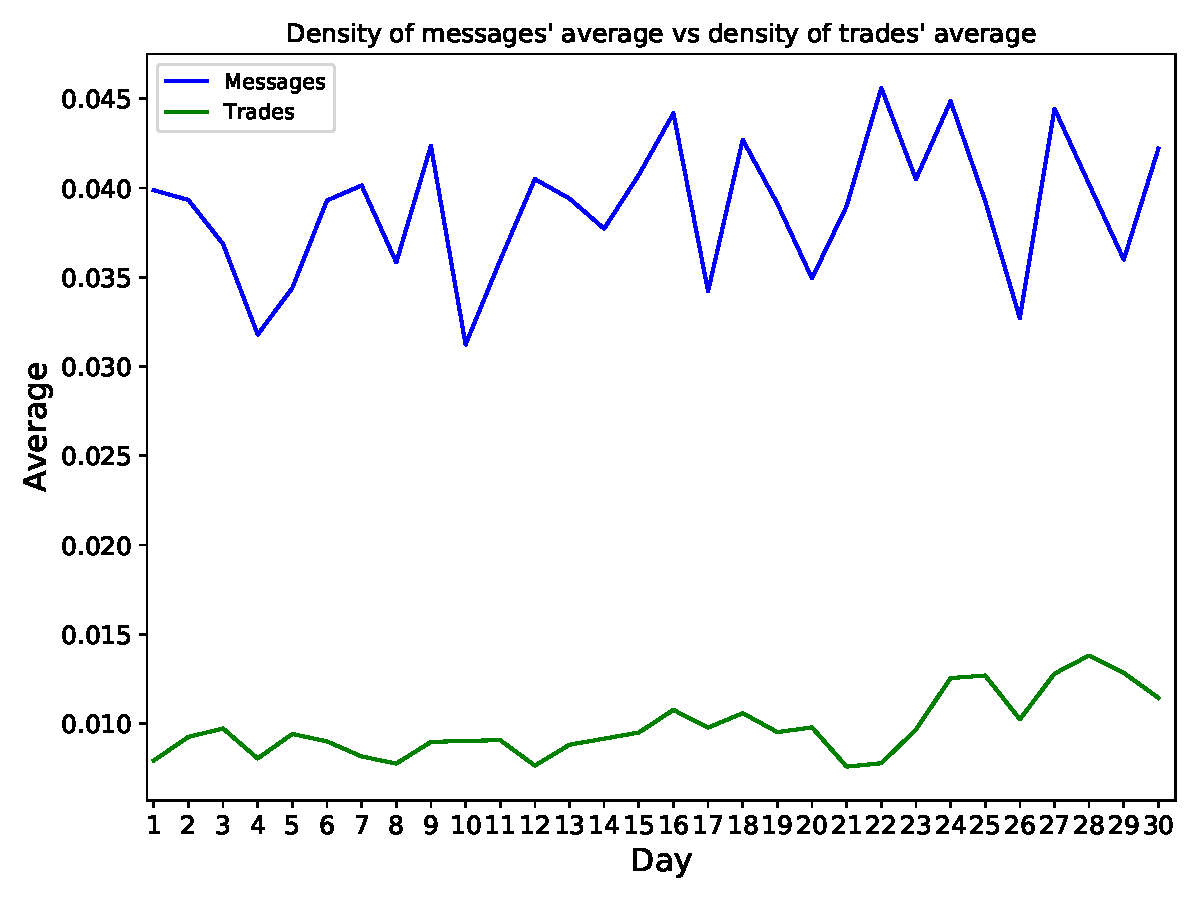
\includegraphics[width=.45\linewidth]{images/Community/Density_Reciprocity/msg_vs_trades_density}
	}
	\hfill
	\subfloat[Reciprocità di messaggi e scambi delle community più rilevanti.]{%
		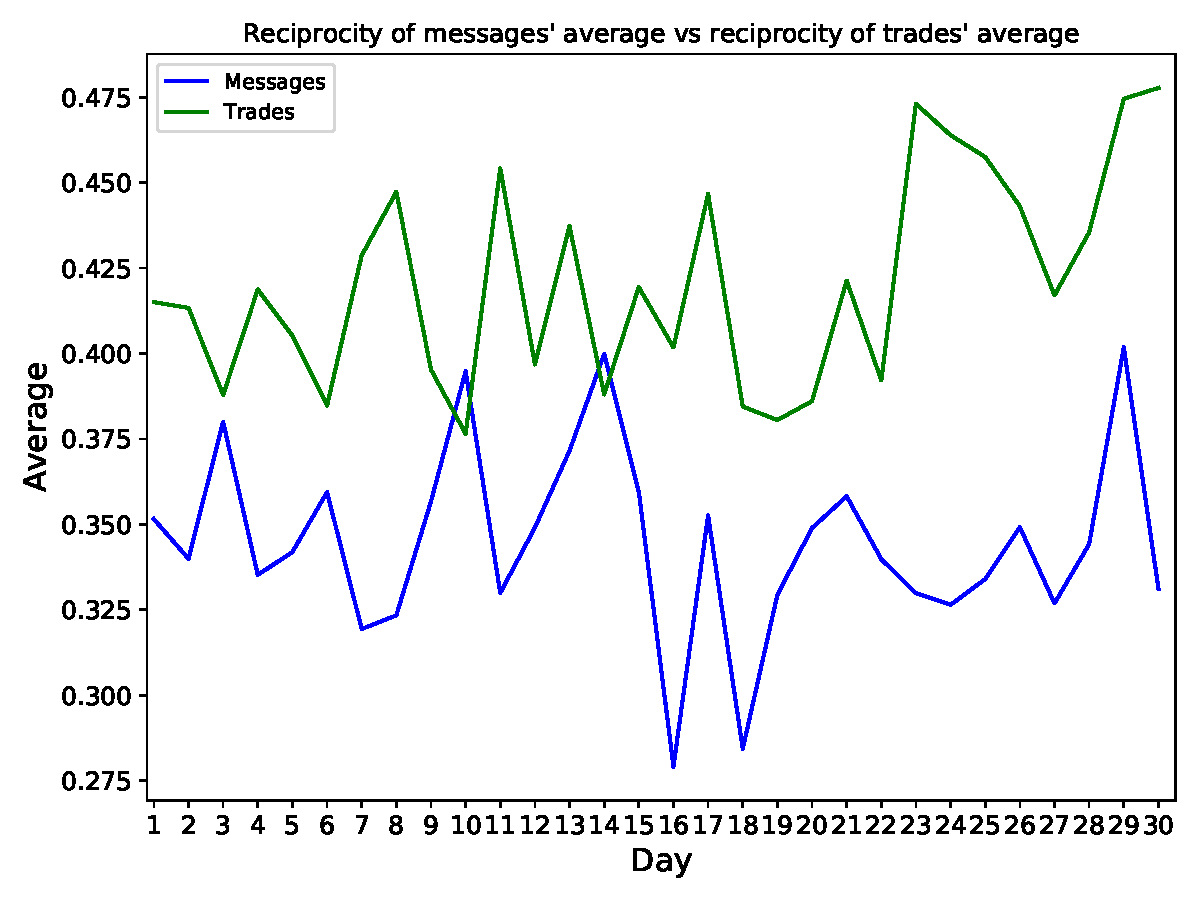
\includegraphics[width=.45\linewidth]{images/Community/Density_Reciprocity/msg_vs_trades_reciprocity}
	}
	\caption{Andamento di densità e reciprocità delle community più rilevanti-}
	\label{fig:density_reciprocity}
\end{figure}

Un'ulteriore analisi compiuta sulle community è il numero di esse che risulta assente (ovvero con densità pari a 0) in uno dei due layer analizzate. Il grafico ottenuto, riportato in Figura \ref{fig:densityzeroper}, mostra come quasi 1 community su 4 sia inattiva a livello degli scambi, mentre i membri circa 1 su 10 non comunicano tra loro all'interno di una giornata. I picchi di inattività, inoltre, corrispondono ad apici negativi nei valori di densità e reciprocità nei grafici in Figura \ref{fig:density_reciprocity}. Ciò e perfettamente ragionevole, in quanto una community con densità zero influisce negativamente sul valore medio della misure per le alleanze.
\begin{figure}
	\centering
	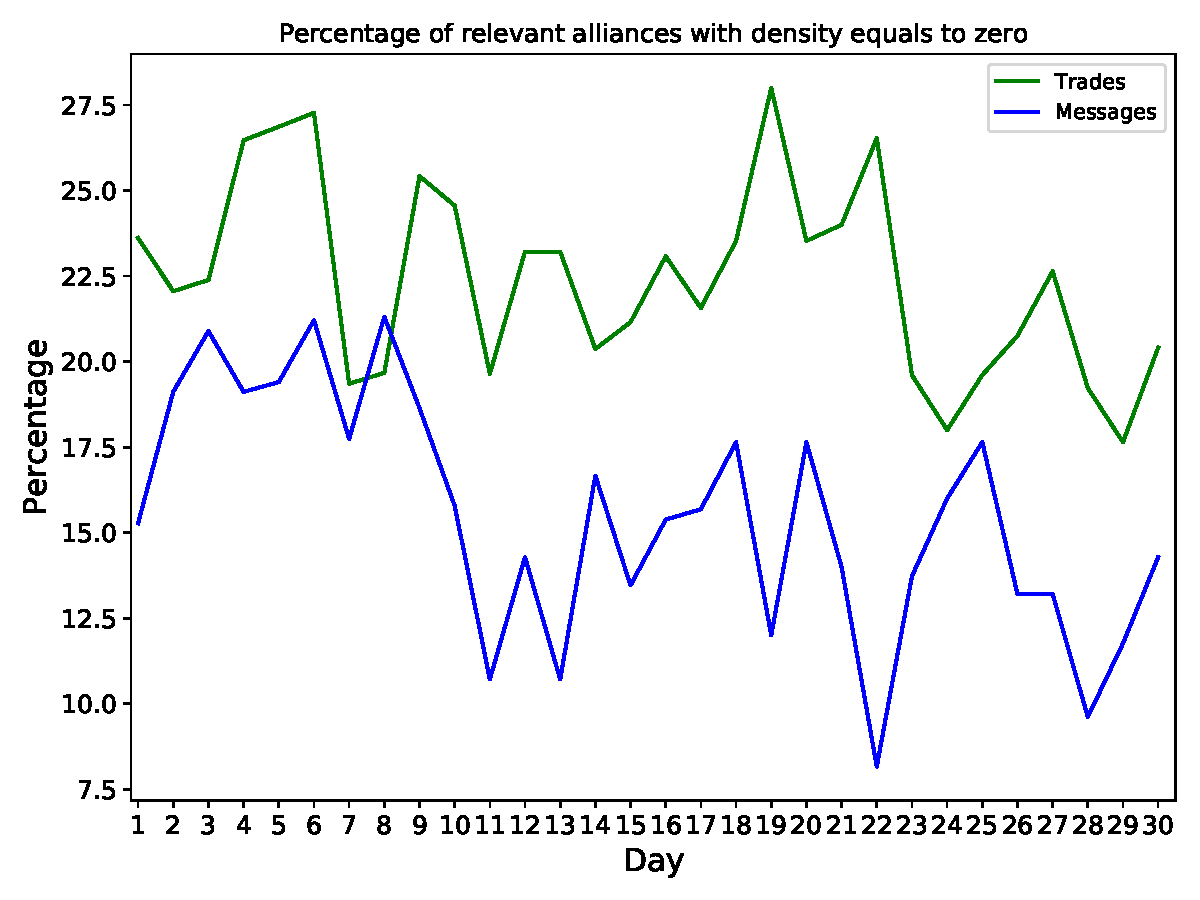
\includegraphics[width=0.9\linewidth]{images/Community/Density_Reciprocity/density_zero_per}
	\caption{Rapporto tra numero di community rilevanti con densità pari a 0 rispetto al numero totale di community rilevanti.}
	\label{fig:densityzeroper}
\end{figure}


\subsection{Analisi della community principale}
Per determinare quale fosse l'alleanza principale (la più rilevante) contenuta nel dataset, abbiamo deciso di utilizzare come metrica la dimensione e la stabilità della community sui 30 giorni. Abbiamo così scelto l'alleanza di dimensione massima e con minore deviazione standard, che si è rivelata essere quella con identificatore 43. Riportiamo inoltre che per le prime 4 community in ordine di grandezza, la dimensione media e la relativa deviazione standard non mostrano differenze statisticamente significative. rispetto alla community scelta. Possiamo quindi immaginare che all'interno del server vi sia un piccolo sottoinsieme di alleanze principali, considerabili molto numerose e stabili, affiancate ad un ben più alto numero di community meno rilevanti e molto più dinamiche, che crescono di dimensione, si scindono o addirittura scompaiono.\\
Per l'analisi della community è stato analizzato il layer delle comunicazioni, in quanto abbiamo ritenuto che fosse quello maggiormente significativo per estrarre analisi interessanti dal punto di vista sociale e del flusso informativo.
Sono state ripetute le misure di centralità trattate nelle Sezioni \ref{subsec:grado} e \ref{subsec:centrality}, con l'aggiunta del calcolo della closeness, ovvero una misura di quanto un nodo sia vicino al flusso informativo presente nella rete. I risultati sono riportati nelle Figure \ref{fig:comm_mean}  e \ref{fig:comm_nodes}, dove sono riportate le distruzioni delle medie delle misure e i valori per ogni nodo nei 30 giorni. Dalle distribuzioni riportare risulta evidente come vi sia una grande maggioranza di membri all'interno dell'alleanza che risultano essere poco influenti, mentre ad una parte minoritaria dei nodi sono associati valori più elevati.\\
Un'analisi approfondita mostra come i valori di centralità sopra la media siano associati in modo ricorrente agli stessi nodi: essi corrispondono probabilmente alle figure più rilevanti all'interno dell'alleanza, quali il leader, i suoi diretti sottoposti e figure come il reclutatore.
Emerge quindi una gestione piramidale della community, con pochi membri ai vertici ed una moltitudine di componenti poco rilevanti.
\begin{figure}
	\begin{tabular}{cc}
		\subfloat[Out degree]{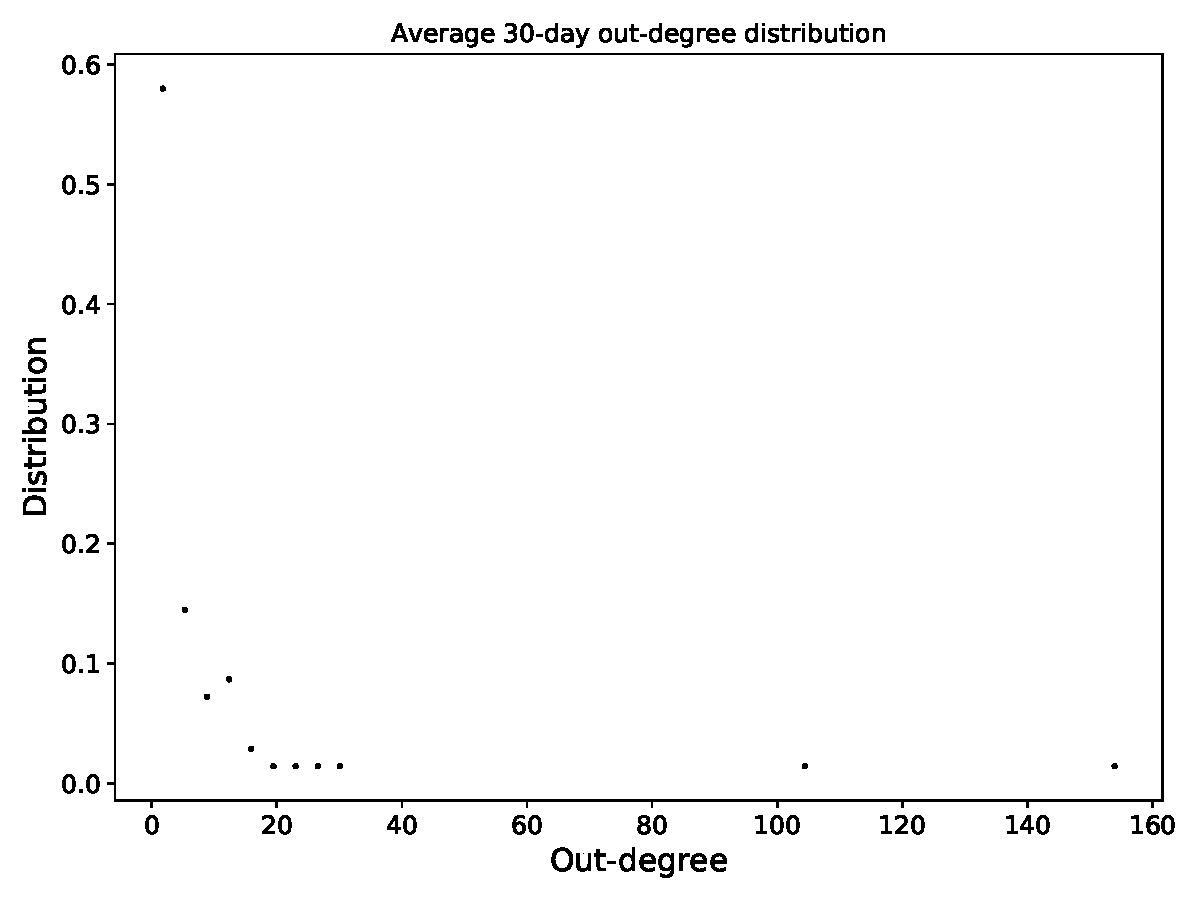
\includegraphics[width = .5\textwidth]{images/Most_important_community/distribution/out-degree_distribution}} &
		\subfloat[Betweenness]{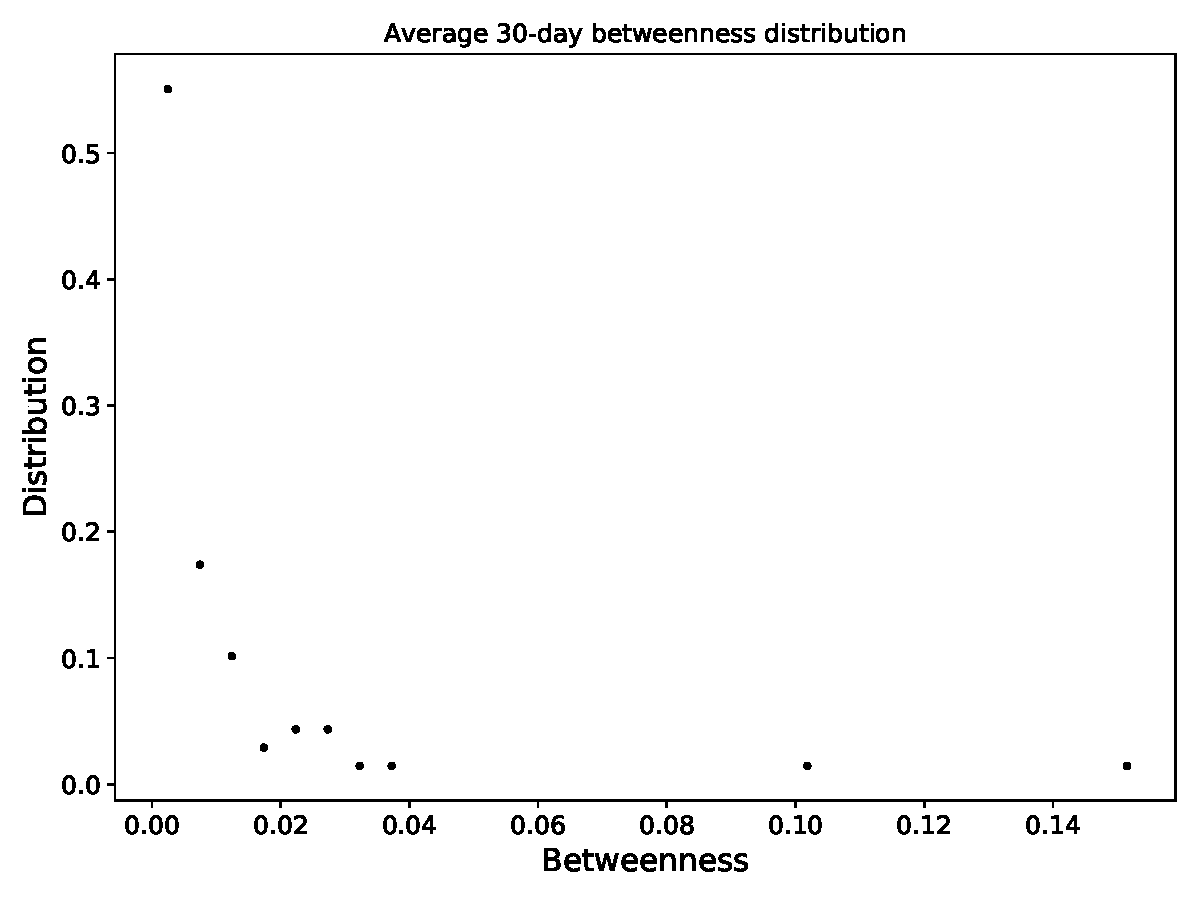
\includegraphics[width = .5\textwidth]{images/Most_important_community/distribution/betweenness_distribution}}\\
		\subfloat[Closeness]{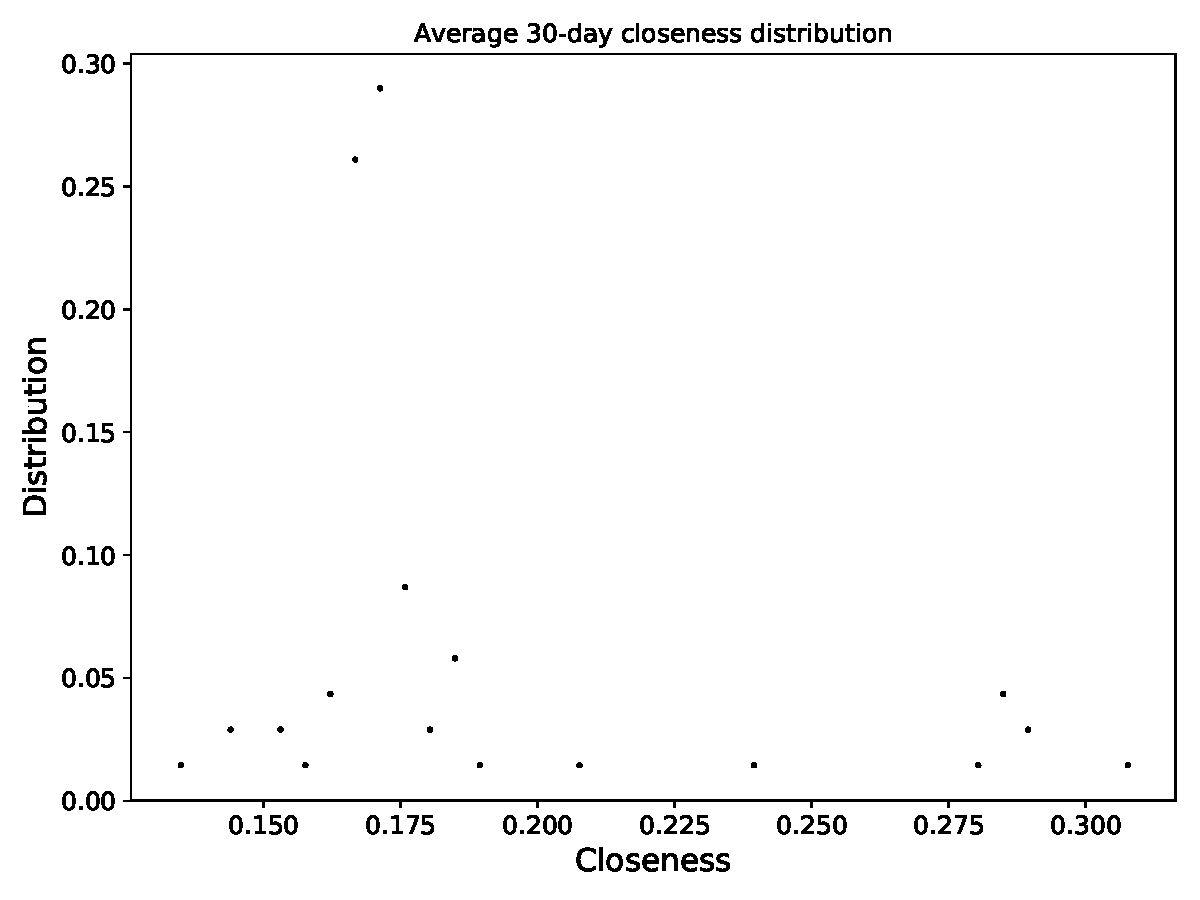
\includegraphics[width = .5\textwidth]{images/Most_important_community/distribution/closeness_distribution}} &
		\subfloat[PageRank]{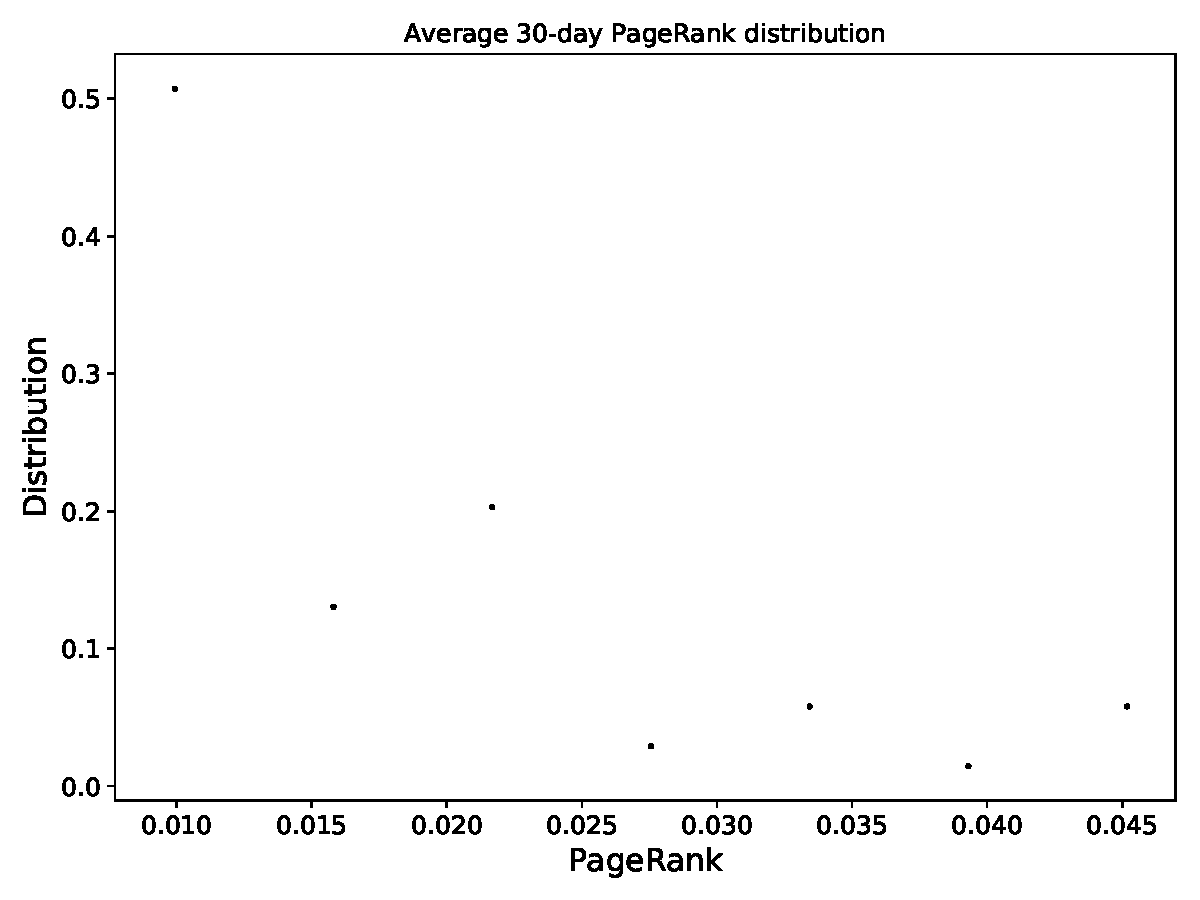
\includegraphics[width = .5\textwidth]{images/Most_important_community/distribution/pagerank_distribution}}
	\end{tabular}
	\caption{Out-degree, Betweenness, Closeness e PageRank medio sui 30 giorni.}
	\label{fig:comm_mean}
\end{figure}
\begin{figure}
	\begin{tabular}{cc}
		\subfloat[Out degree]{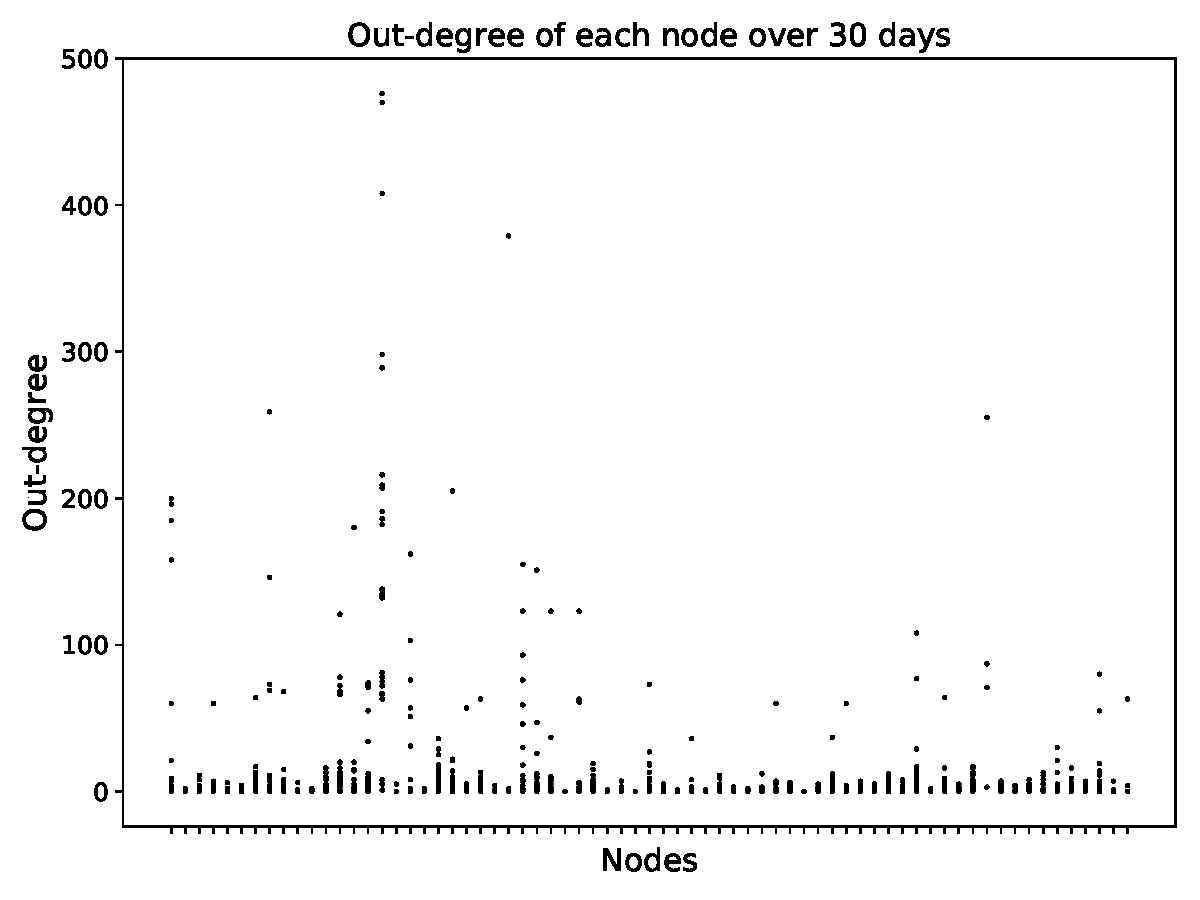
\includegraphics[width = .5\textwidth]{images/Most_important_community/each_node/out-degree_each_node}} &
		\subfloat[Betweenness]{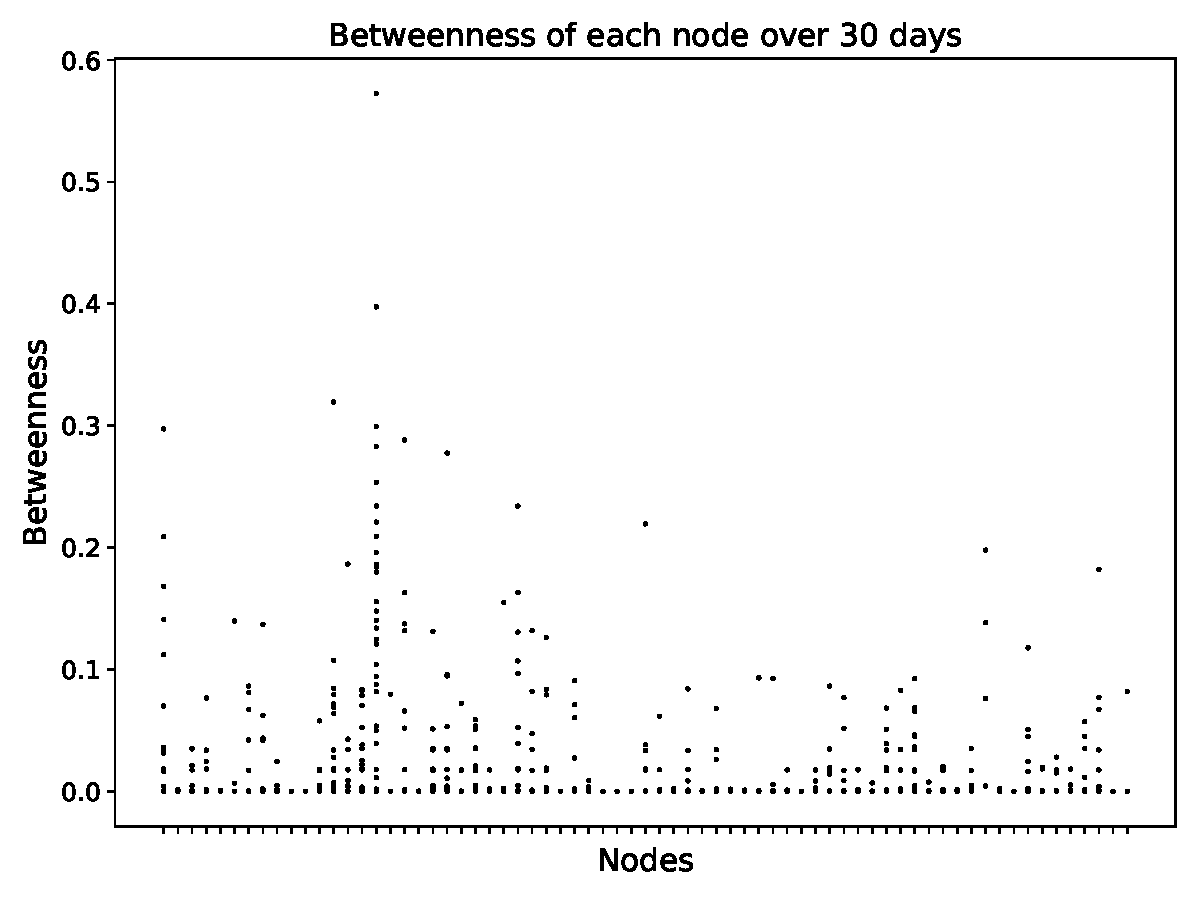
\includegraphics[width = .5\textwidth]{images/Most_important_community/each_node/betweenness_each_node}}\\
		\subfloat[Closeness]{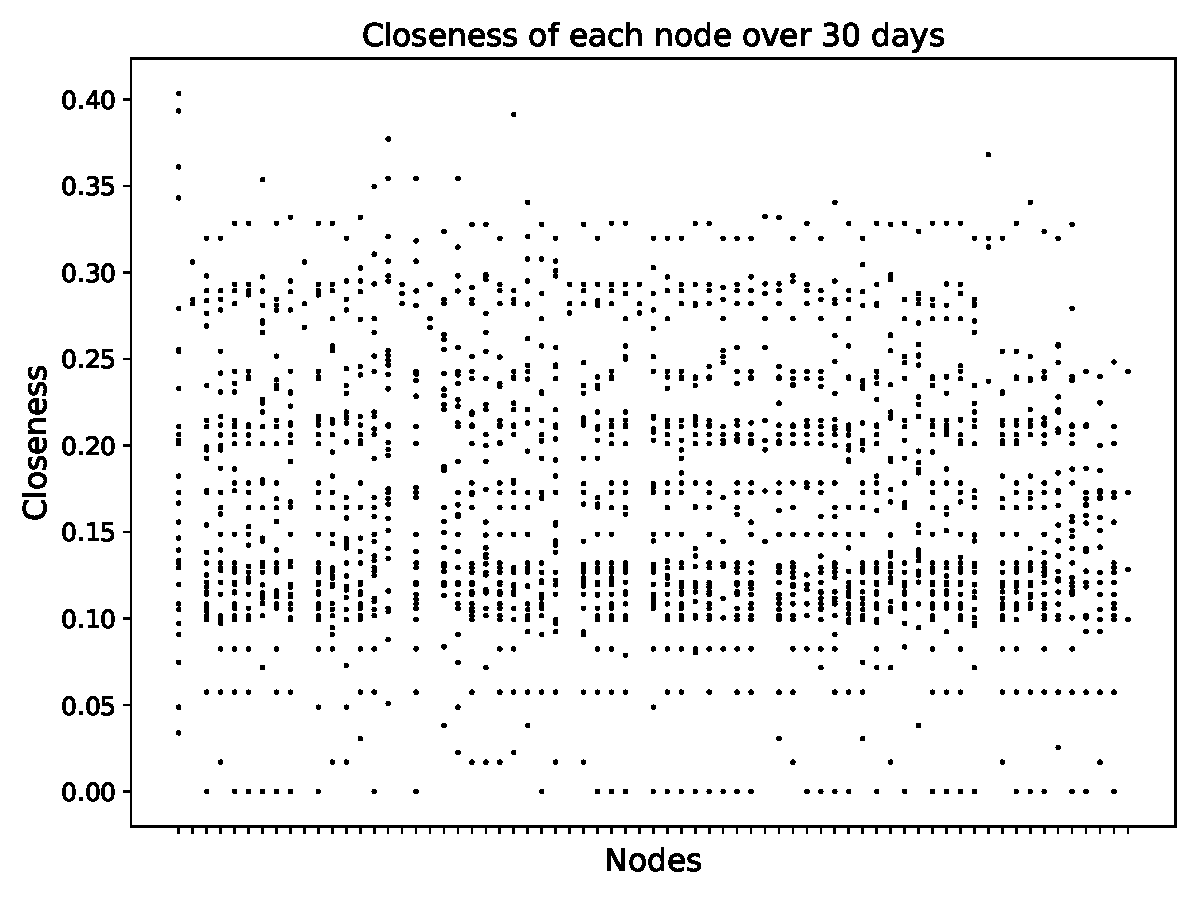
\includegraphics[width = .5\textwidth]{images/Most_important_community/each_node/closeness_each_node}} &
		\subfloat[PageRank]{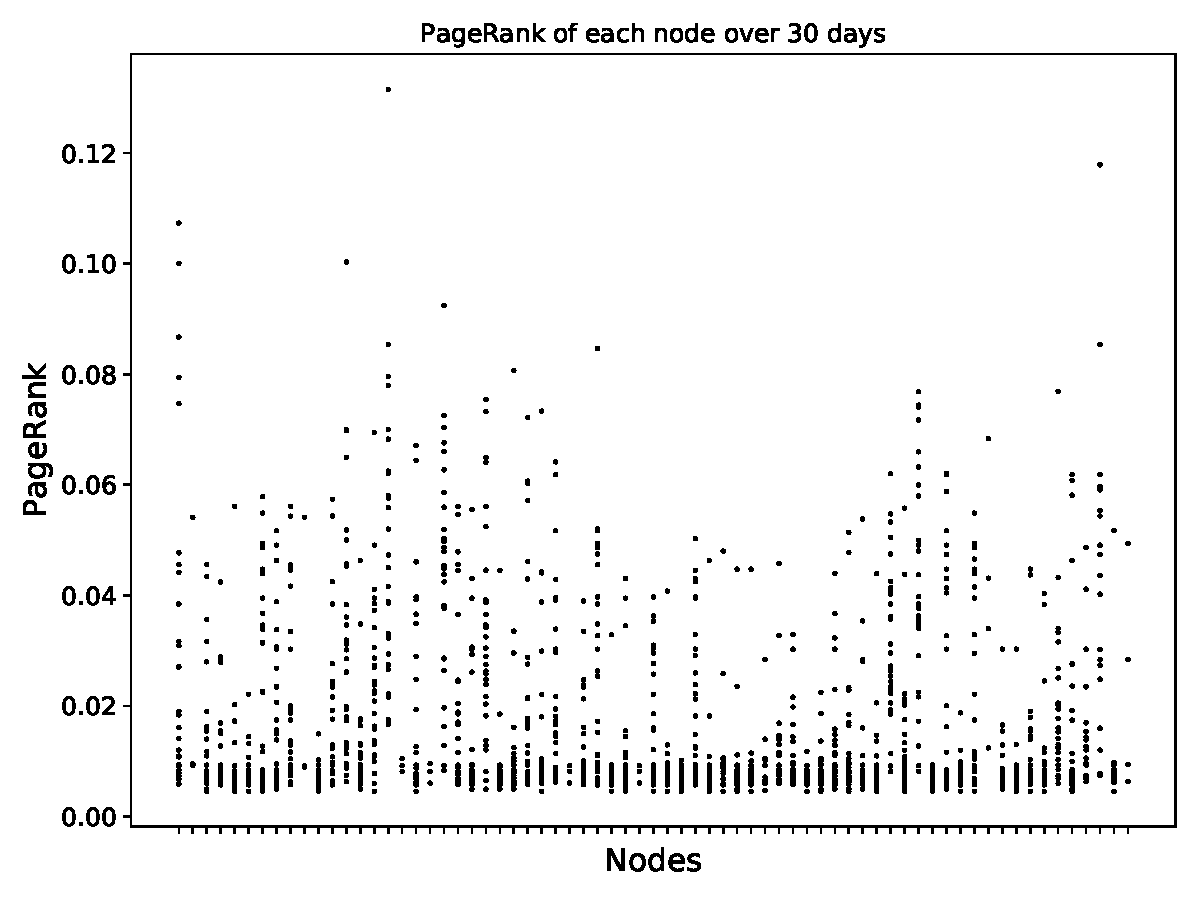
\includegraphics[width = .5\textwidth]{images/Most_important_community/each_node/pagerank_each_node}}
	\end{tabular}
	\caption{Out-degree, Betweenness, Closeness e PageRank di ogni nodo dell'alleanza principale per ognuno dei 30 giorni.}
	\label{fig:comm_nodes}
\end{figure}

Abbiamo poi analizzato i valori di densità e di reciprocità di questa community e li abbiamo confrontati con i valori medi ottenuti nella Sezione \ref{sec:density}, cercando di stabilire se vi fossero differenze rilevanti. Le Figure \ref{fig:most_imp_mess} e \ref{fig:most_imp_trade} mostrano valori di densità e reciprocità dei trade nettamente maggiori all'interno di questa alleanza rispetto alla media delle altre community. Lo stesso vale per la densità dei messaggi, mentre per quanto riguarda la reciprocità troviamo valori lievemente inferiori rispetto alla media, con picchi di positivi in alcuni giorni. Questo tipo di dato può essere causato, come già affermato precedentemente, dalla mancanza nel dataset dei messaggi di \textit{broadcast}, utilizzati per le comunicazioni da parte dei membri di alto grado dell'alleanza. L'immagine che emerge da questa analisi è quella di una community più coesa della media, con una discreta attività di scambi e commerci interni alla community che va oltre la media delle community concorrenti.
\begin{figure}
	\subfloat[Confronto tra densità di messaggi della community analizzata rispetto alla media.]{%
		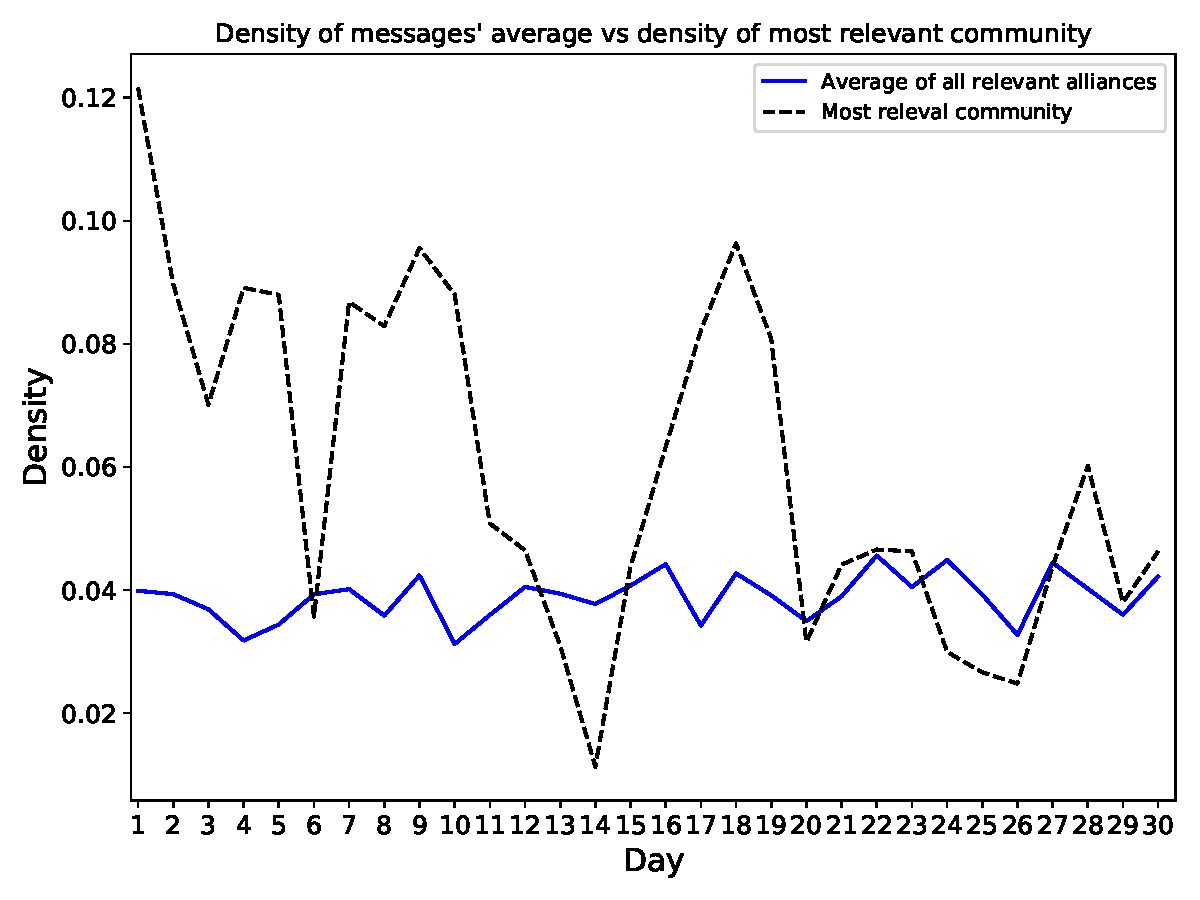
\includegraphics[width=.45\linewidth]{images/Most_important_community/density/msg_vs_most_density}
	}
	\hfill
	\subfloat[Confronto tra reciprocità dei messaggi della community analizzata rispetto alla media.]{%
		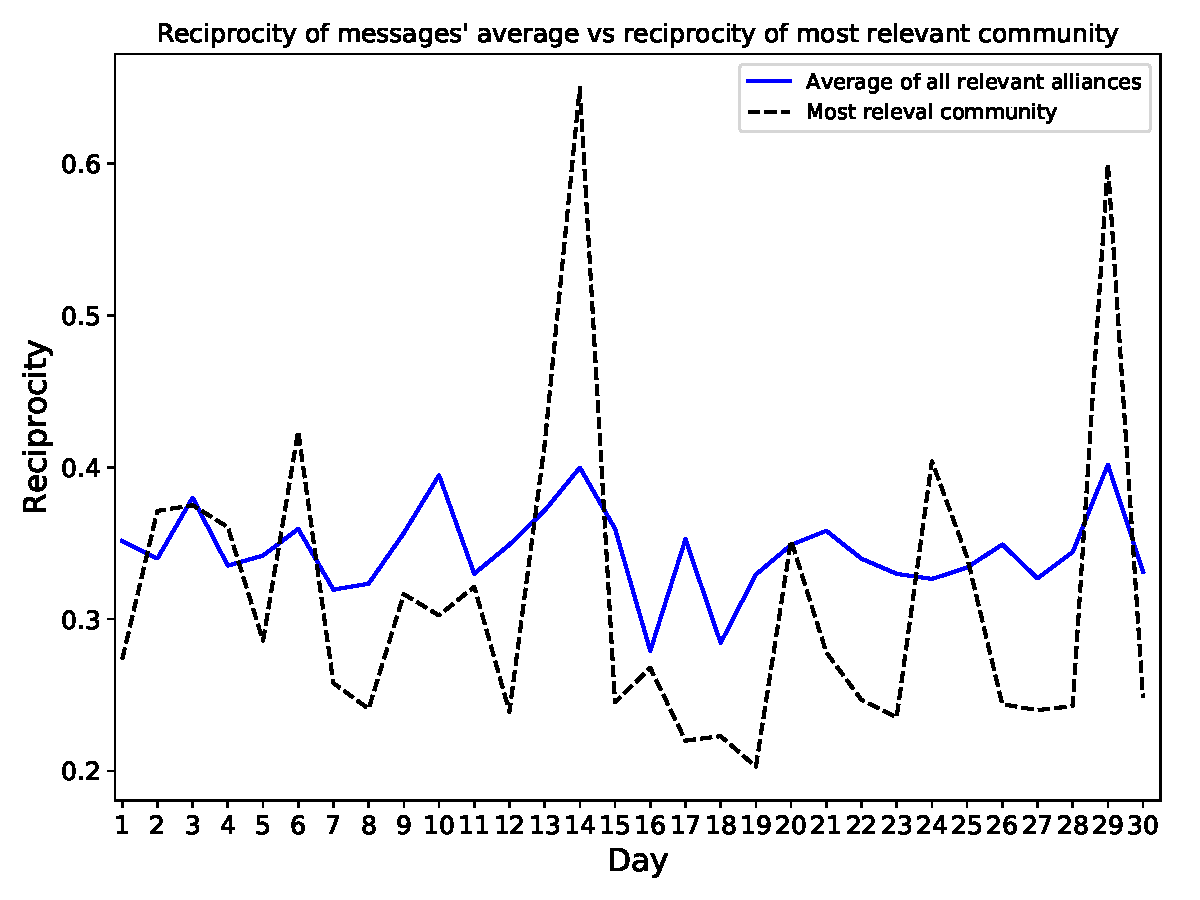
\includegraphics[width=.45\linewidth]{images/Most_important_community/density/msg_vs_most_reciprocity}
	}
	\caption{Andamento di densità e reciprocità dei messaggi della community a confronto con le medie della rete.}
	\label{fig:most_imp_mess}
\end{figure}
\begin{figure}
	\subfloat[Confronto tra densità di trade della community analizzata rispetto alla media.]{%
		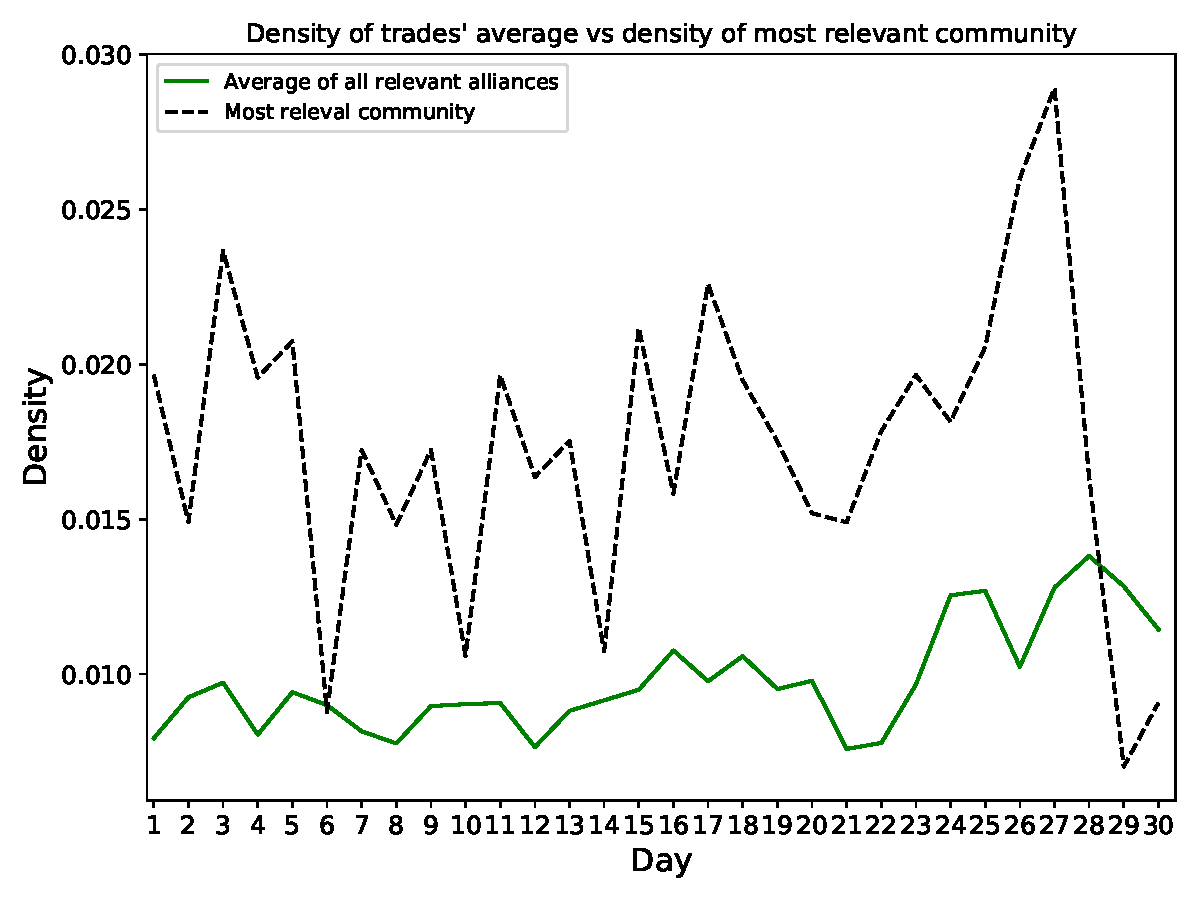
\includegraphics[width=.45\linewidth]{images/Most_important_community/density/trades_vs_most_density}
	}
	\hfill
	\subfloat[Confronto tra reciprocità dei trade della community analizzata rispetto alla media.]{%
		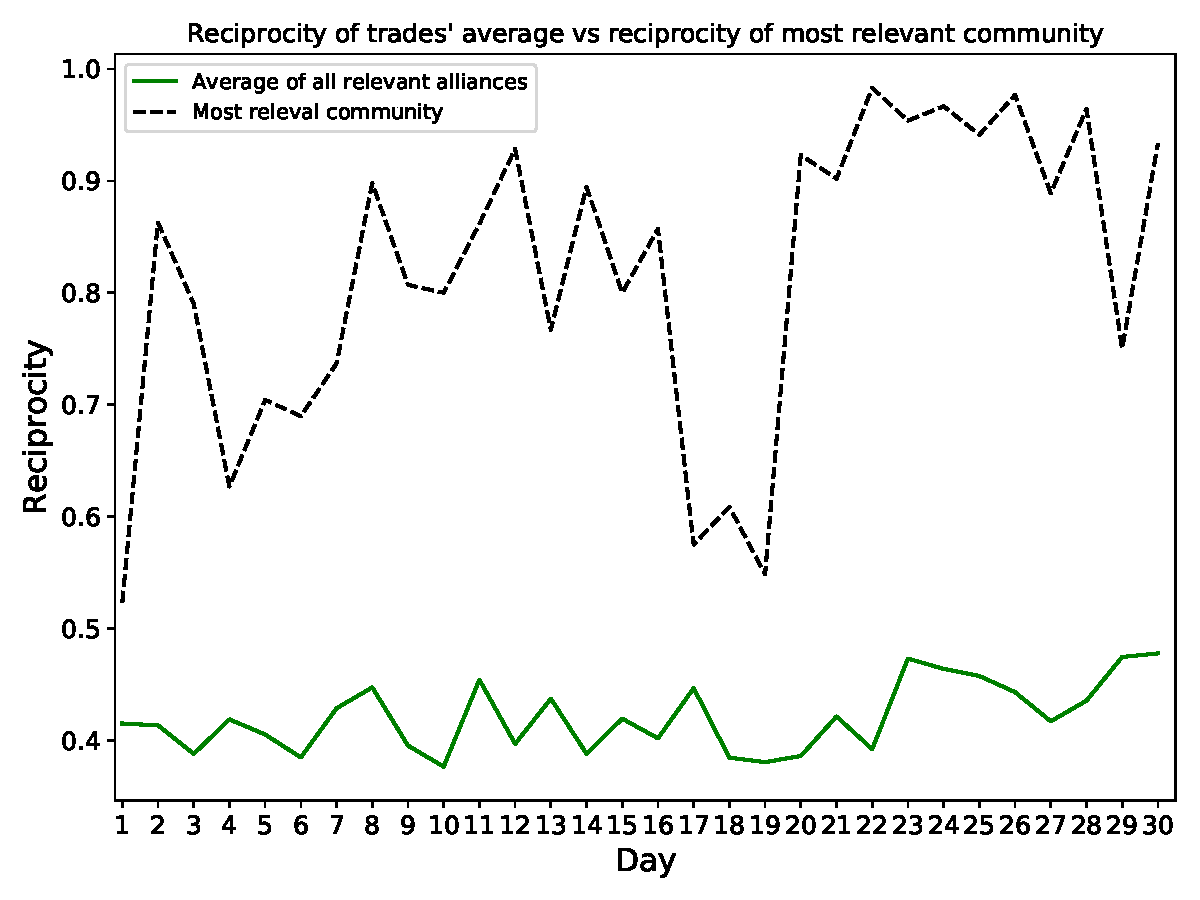
\includegraphics[width=.45\linewidth]{images/Most_important_community/density/trades_vs_most_reciprocity}
	}
	\caption{Andamento di densità e reciprocità dei trade della community a confronto con i valori medi delle community.}
	\label{fig:most_imp_trade}
\end{figure}

\newpage
\subsection{Evoluzione nel tempo}
Come affermato nella Sezione precedente, il server è costituito da un grande numero di alleanze registrate, ma quante di queste sono davvero da considerarsi come influenti? Abbiamo quindi indagato come il numero di alleanze registrate variasse nel tempo, cercando di identificare se vi fosse un chiaro trand di accorpamento delle community o di disaggregazione di esse. I risultati ottenuto, mostrati in Figura \ref{fig:allianceseachday}, mostrano una progressiva diminuzione sia del numero di alleanze totale, sia del numero di alleanze considerabili rilevanti (si ricorda che come metrica di rilevanza è stata utilizzato il numero minimo di membri pari a 10). La percentuale di community rilevanti sul totale si mantiene pressochè stabile, oscillando tra il $25\%$ e il $35\%$.\\
L'andamento decrescente mostrato in Figura \ref{fig:allianceseachday} sembra confermare il trand presente anche nelle Figure \ref{fig:activity_each_day} e \ref{fig:playereachday}, che mostra un progressivo spopolamento del server, con conseguente diminuzione del numero di attività totali eseguite ogni giorno.\\
Data la presenza ricorrente in questi grafici di un picco negativo al giorno 5, abbiamo deciso di indagare più approfonditamente questo fenomeno, sospettando che un qualche intervento esterno potesse aver alterato il numero di giocatori presenti. Analizzando gli insiemi dei giocatori presenti prima e dopo il quinto giorno, abbiamo rilevato che ben 715 giocatori che erano presenti in almeno uno dei layer della rete nei gironi precedenti al crollo, non hanno compiuto alcun tipo di attività nei successivi 25 giorni! Questo tipo di riscontro sembrerebbe essere compatibile con un evento esterno che abbia rimosso i giocatori (\textit{e.g.}, ban) o che li abbia portati ad andarsene (\textit{e.g.}, apertura di un nuovo server). Sfortunatamente non siamo riusciti a trovare conferme di queste ipotesi, in quanto non siamo riusciti a trovare alcuna prova online che confermasse o smentisse la nostra tesi.
\begin{figure}
	\centering
	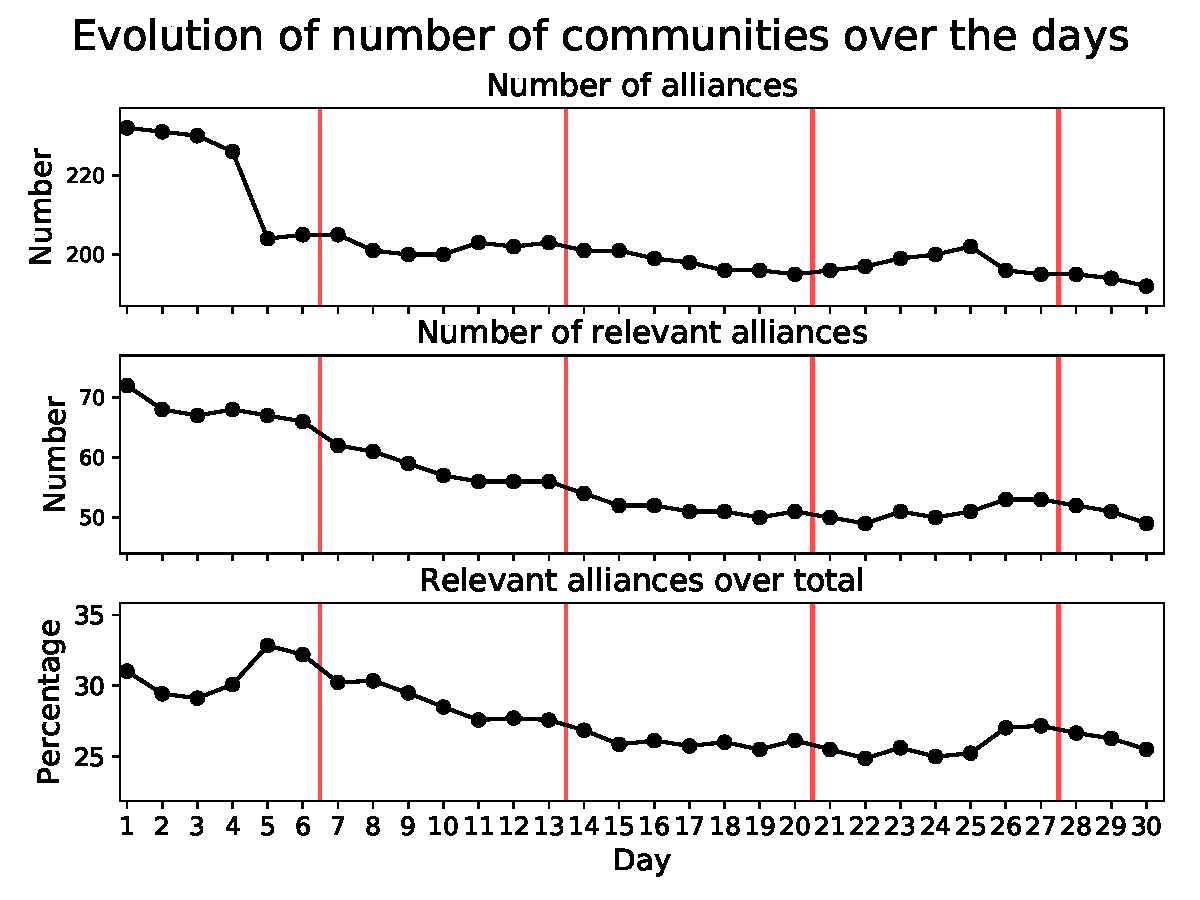
\includegraphics[width=0.85\linewidth]{images/alliances_each_day}
	\caption{Andamento del numero di community registrate nel tempo.}
	\label{fig:allianceseachday}
\end{figure}


\subsection{Interazioni tra le alleanze}
